
% Default to the notebook output style

    


% Inherit from the specified cell style.




    
\documentclass[11pt]{article}

    
    
    \usepackage[T1]{fontenc}
    % Nicer default font (+ math font) than Computer Modern for most use cases
    \usepackage{mathpazo}

    % Basic figure setup, for now with no caption control since it's done
    % automatically by Pandoc (which extracts ![](path) syntax from Markdown).
    \usepackage{graphicx}
    % We will generate all images so they have a width \maxwidth. This means
    % that they will get their normal width if they fit onto the page, but
    % are scaled down if they would overflow the margins.
    \makeatletter
    \def\maxwidth{\ifdim\Gin@nat@width>\linewidth\linewidth
    \else\Gin@nat@width\fi}
    \makeatother
    \let\Oldincludegraphics\includegraphics
    % Set max figure width to be 80% of text width, for now hardcoded.
    \renewcommand{\includegraphics}[1]{\Oldincludegraphics[width=.8\maxwidth]{#1}}
    % Ensure that by default, figures have no caption (until we provide a
    % proper Figure object with a Caption API and a way to capture that
    % in the conversion process - todo).
    \usepackage{caption}
    \DeclareCaptionLabelFormat{nolabel}{}
    \captionsetup{labelformat=nolabel}

    \usepackage{adjustbox} % Used to constrain images to a maximum size 
    \usepackage{xcolor} % Allow colors to be defined
    \usepackage{enumerate} % Needed for markdown enumerations to work
    \usepackage{geometry} % Used to adjust the document margins
    \usepackage{amsmath} % Equations
    \usepackage{amssymb} % Equations
    \usepackage{textcomp} % defines textquotesingle
    % Hack from http://tex.stackexchange.com/a/47451/13684:
    \AtBeginDocument{%
        \def\PYZsq{\textquotesingle}% Upright quotes in Pygmentized code
    }
    \usepackage{upquote} % Upright quotes for verbatim code
    \usepackage{eurosym} % defines \euro
    \usepackage[mathletters]{ucs} % Extended unicode (utf-8) support
    \usepackage[utf8x]{inputenc} % Allow utf-8 characters in the tex document
    \usepackage{fancyvrb} % verbatim replacement that allows latex
    \usepackage{grffile} % extends the file name processing of package graphics 
                         % to support a larger range 
    % The hyperref package gives us a pdf with properly built
    % internal navigation ('pdf bookmarks' for the table of contents,
    % internal cross-reference links, web links for URLs, etc.)
    \usepackage{hyperref}
    \usepackage{longtable} % longtable support required by pandoc >1.10
    \usepackage{booktabs}  % table support for pandoc > 1.12.2
    \usepackage[inline]{enumitem} % IRkernel/repr support (it uses the enumerate* environment)
    \usepackage[normalem]{ulem} % ulem is needed to support strikethroughs (\sout)
                                % normalem makes italics be italics, not underlines
    

    
    
    % Colors for the hyperref package
    \definecolor{urlcolor}{rgb}{0,.145,.698}
    \definecolor{linkcolor}{rgb}{.71,0.21,0.01}
    \definecolor{citecolor}{rgb}{.12,.54,.11}

    % ANSI colors
    \definecolor{ansi-black}{HTML}{3E424D}
    \definecolor{ansi-black-intense}{HTML}{282C36}
    \definecolor{ansi-red}{HTML}{E75C58}
    \definecolor{ansi-red-intense}{HTML}{B22B31}
    \definecolor{ansi-green}{HTML}{00A250}
    \definecolor{ansi-green-intense}{HTML}{007427}
    \definecolor{ansi-yellow}{HTML}{DDB62B}
    \definecolor{ansi-yellow-intense}{HTML}{B27D12}
    \definecolor{ansi-blue}{HTML}{208FFB}
    \definecolor{ansi-blue-intense}{HTML}{0065CA}
    \definecolor{ansi-magenta}{HTML}{D160C4}
    \definecolor{ansi-magenta-intense}{HTML}{A03196}
    \definecolor{ansi-cyan}{HTML}{60C6C8}
    \definecolor{ansi-cyan-intense}{HTML}{258F8F}
    \definecolor{ansi-white}{HTML}{C5C1B4}
    \definecolor{ansi-white-intense}{HTML}{A1A6B2}

    % commands and environments needed by pandoc snippets
    % extracted from the output of `pandoc -s`
    \providecommand{\tightlist}{%
      \setlength{\itemsep}{0pt}\setlength{\parskip}{0pt}}
    \DefineVerbatimEnvironment{Highlighting}{Verbatim}{commandchars=\\\{\}}
    % Add ',fontsize=\small' for more characters per line
    \newenvironment{Shaded}{}{}
    \newcommand{\KeywordTok}[1]{\textcolor[rgb]{0.00,0.44,0.13}{\textbf{{#1}}}}
    \newcommand{\DataTypeTok}[1]{\textcolor[rgb]{0.56,0.13,0.00}{{#1}}}
    \newcommand{\DecValTok}[1]{\textcolor[rgb]{0.25,0.63,0.44}{{#1}}}
    \newcommand{\BaseNTok}[1]{\textcolor[rgb]{0.25,0.63,0.44}{{#1}}}
    \newcommand{\FloatTok}[1]{\textcolor[rgb]{0.25,0.63,0.44}{{#1}}}
    \newcommand{\CharTok}[1]{\textcolor[rgb]{0.25,0.44,0.63}{{#1}}}
    \newcommand{\StringTok}[1]{\textcolor[rgb]{0.25,0.44,0.63}{{#1}}}
    \newcommand{\CommentTok}[1]{\textcolor[rgb]{0.38,0.63,0.69}{\textit{{#1}}}}
    \newcommand{\OtherTok}[1]{\textcolor[rgb]{0.00,0.44,0.13}{{#1}}}
    \newcommand{\AlertTok}[1]{\textcolor[rgb]{1.00,0.00,0.00}{\textbf{{#1}}}}
    \newcommand{\FunctionTok}[1]{\textcolor[rgb]{0.02,0.16,0.49}{{#1}}}
    \newcommand{\RegionMarkerTok}[1]{{#1}}
    \newcommand{\ErrorTok}[1]{\textcolor[rgb]{1.00,0.00,0.00}{\textbf{{#1}}}}
    \newcommand{\NormalTok}[1]{{#1}}
    
    % Additional commands for more recent versions of Pandoc
    \newcommand{\ConstantTok}[1]{\textcolor[rgb]{0.53,0.00,0.00}{{#1}}}
    \newcommand{\SpecialCharTok}[1]{\textcolor[rgb]{0.25,0.44,0.63}{{#1}}}
    \newcommand{\VerbatimStringTok}[1]{\textcolor[rgb]{0.25,0.44,0.63}{{#1}}}
    \newcommand{\SpecialStringTok}[1]{\textcolor[rgb]{0.73,0.40,0.53}{{#1}}}
    \newcommand{\ImportTok}[1]{{#1}}
    \newcommand{\DocumentationTok}[1]{\textcolor[rgb]{0.73,0.13,0.13}{\textit{{#1}}}}
    \newcommand{\AnnotationTok}[1]{\textcolor[rgb]{0.38,0.63,0.69}{\textbf{\textit{{#1}}}}}
    \newcommand{\CommentVarTok}[1]{\textcolor[rgb]{0.38,0.63,0.69}{\textbf{\textit{{#1}}}}}
    \newcommand{\VariableTok}[1]{\textcolor[rgb]{0.10,0.09,0.49}{{#1}}}
    \newcommand{\ControlFlowTok}[1]{\textcolor[rgb]{0.00,0.44,0.13}{\textbf{{#1}}}}
    \newcommand{\OperatorTok}[1]{\textcolor[rgb]{0.40,0.40,0.40}{{#1}}}
    \newcommand{\BuiltInTok}[1]{{#1}}
    \newcommand{\ExtensionTok}[1]{{#1}}
    \newcommand{\PreprocessorTok}[1]{\textcolor[rgb]{0.74,0.48,0.00}{{#1}}}
    \newcommand{\AttributeTok}[1]{\textcolor[rgb]{0.49,0.56,0.16}{{#1}}}
    \newcommand{\InformationTok}[1]{\textcolor[rgb]{0.38,0.63,0.69}{\textbf{\textit{{#1}}}}}
    \newcommand{\WarningTok}[1]{\textcolor[rgb]{0.38,0.63,0.69}{\textbf{\textit{{#1}}}}}
    
    
    % Define a nice break command that doesn't care if a line doesn't already
    % exist.
    \def\br{\hspace*{\fill} \\* }
    % Math Jax compatability definitions
    \def\gt{>}
    \def\lt{<}
    % Document parameters
    \title{TP\_Modelisation}
    
    
    

    % Pygments definitions
    
\makeatletter
\def\PY@reset{\let\PY@it=\relax \let\PY@bf=\relax%
    \let\PY@ul=\relax \let\PY@tc=\relax%
    \let\PY@bc=\relax \let\PY@ff=\relax}
\def\PY@tok#1{\csname PY@tok@#1\endcsname}
\def\PY@toks#1+{\ifx\relax#1\empty\else%
    \PY@tok{#1}\expandafter\PY@toks\fi}
\def\PY@do#1{\PY@bc{\PY@tc{\PY@ul{%
    \PY@it{\PY@bf{\PY@ff{#1}}}}}}}
\def\PY#1#2{\PY@reset\PY@toks#1+\relax+\PY@do{#2}}

\expandafter\def\csname PY@tok@w\endcsname{\def\PY@tc##1{\textcolor[rgb]{0.73,0.73,0.73}{##1}}}
\expandafter\def\csname PY@tok@c\endcsname{\let\PY@it=\textit\def\PY@tc##1{\textcolor[rgb]{0.25,0.50,0.50}{##1}}}
\expandafter\def\csname PY@tok@cp\endcsname{\def\PY@tc##1{\textcolor[rgb]{0.74,0.48,0.00}{##1}}}
\expandafter\def\csname PY@tok@k\endcsname{\let\PY@bf=\textbf\def\PY@tc##1{\textcolor[rgb]{0.00,0.50,0.00}{##1}}}
\expandafter\def\csname PY@tok@kp\endcsname{\def\PY@tc##1{\textcolor[rgb]{0.00,0.50,0.00}{##1}}}
\expandafter\def\csname PY@tok@kt\endcsname{\def\PY@tc##1{\textcolor[rgb]{0.69,0.00,0.25}{##1}}}
\expandafter\def\csname PY@tok@o\endcsname{\def\PY@tc##1{\textcolor[rgb]{0.40,0.40,0.40}{##1}}}
\expandafter\def\csname PY@tok@ow\endcsname{\let\PY@bf=\textbf\def\PY@tc##1{\textcolor[rgb]{0.67,0.13,1.00}{##1}}}
\expandafter\def\csname PY@tok@nb\endcsname{\def\PY@tc##1{\textcolor[rgb]{0.00,0.50,0.00}{##1}}}
\expandafter\def\csname PY@tok@nf\endcsname{\def\PY@tc##1{\textcolor[rgb]{0.00,0.00,1.00}{##1}}}
\expandafter\def\csname PY@tok@nc\endcsname{\let\PY@bf=\textbf\def\PY@tc##1{\textcolor[rgb]{0.00,0.00,1.00}{##1}}}
\expandafter\def\csname PY@tok@nn\endcsname{\let\PY@bf=\textbf\def\PY@tc##1{\textcolor[rgb]{0.00,0.00,1.00}{##1}}}
\expandafter\def\csname PY@tok@ne\endcsname{\let\PY@bf=\textbf\def\PY@tc##1{\textcolor[rgb]{0.82,0.25,0.23}{##1}}}
\expandafter\def\csname PY@tok@nv\endcsname{\def\PY@tc##1{\textcolor[rgb]{0.10,0.09,0.49}{##1}}}
\expandafter\def\csname PY@tok@no\endcsname{\def\PY@tc##1{\textcolor[rgb]{0.53,0.00,0.00}{##1}}}
\expandafter\def\csname PY@tok@nl\endcsname{\def\PY@tc##1{\textcolor[rgb]{0.63,0.63,0.00}{##1}}}
\expandafter\def\csname PY@tok@ni\endcsname{\let\PY@bf=\textbf\def\PY@tc##1{\textcolor[rgb]{0.60,0.60,0.60}{##1}}}
\expandafter\def\csname PY@tok@na\endcsname{\def\PY@tc##1{\textcolor[rgb]{0.49,0.56,0.16}{##1}}}
\expandafter\def\csname PY@tok@nt\endcsname{\let\PY@bf=\textbf\def\PY@tc##1{\textcolor[rgb]{0.00,0.50,0.00}{##1}}}
\expandafter\def\csname PY@tok@nd\endcsname{\def\PY@tc##1{\textcolor[rgb]{0.67,0.13,1.00}{##1}}}
\expandafter\def\csname PY@tok@s\endcsname{\def\PY@tc##1{\textcolor[rgb]{0.73,0.13,0.13}{##1}}}
\expandafter\def\csname PY@tok@sd\endcsname{\let\PY@it=\textit\def\PY@tc##1{\textcolor[rgb]{0.73,0.13,0.13}{##1}}}
\expandafter\def\csname PY@tok@si\endcsname{\let\PY@bf=\textbf\def\PY@tc##1{\textcolor[rgb]{0.73,0.40,0.53}{##1}}}
\expandafter\def\csname PY@tok@se\endcsname{\let\PY@bf=\textbf\def\PY@tc##1{\textcolor[rgb]{0.73,0.40,0.13}{##1}}}
\expandafter\def\csname PY@tok@sr\endcsname{\def\PY@tc##1{\textcolor[rgb]{0.73,0.40,0.53}{##1}}}
\expandafter\def\csname PY@tok@ss\endcsname{\def\PY@tc##1{\textcolor[rgb]{0.10,0.09,0.49}{##1}}}
\expandafter\def\csname PY@tok@sx\endcsname{\def\PY@tc##1{\textcolor[rgb]{0.00,0.50,0.00}{##1}}}
\expandafter\def\csname PY@tok@m\endcsname{\def\PY@tc##1{\textcolor[rgb]{0.40,0.40,0.40}{##1}}}
\expandafter\def\csname PY@tok@gh\endcsname{\let\PY@bf=\textbf\def\PY@tc##1{\textcolor[rgb]{0.00,0.00,0.50}{##1}}}
\expandafter\def\csname PY@tok@gu\endcsname{\let\PY@bf=\textbf\def\PY@tc##1{\textcolor[rgb]{0.50,0.00,0.50}{##1}}}
\expandafter\def\csname PY@tok@gd\endcsname{\def\PY@tc##1{\textcolor[rgb]{0.63,0.00,0.00}{##1}}}
\expandafter\def\csname PY@tok@gi\endcsname{\def\PY@tc##1{\textcolor[rgb]{0.00,0.63,0.00}{##1}}}
\expandafter\def\csname PY@tok@gr\endcsname{\def\PY@tc##1{\textcolor[rgb]{1.00,0.00,0.00}{##1}}}
\expandafter\def\csname PY@tok@ge\endcsname{\let\PY@it=\textit}
\expandafter\def\csname PY@tok@gs\endcsname{\let\PY@bf=\textbf}
\expandafter\def\csname PY@tok@gp\endcsname{\let\PY@bf=\textbf\def\PY@tc##1{\textcolor[rgb]{0.00,0.00,0.50}{##1}}}
\expandafter\def\csname PY@tok@go\endcsname{\def\PY@tc##1{\textcolor[rgb]{0.53,0.53,0.53}{##1}}}
\expandafter\def\csname PY@tok@gt\endcsname{\def\PY@tc##1{\textcolor[rgb]{0.00,0.27,0.87}{##1}}}
\expandafter\def\csname PY@tok@err\endcsname{\def\PY@bc##1{\setlength{\fboxsep}{0pt}\fcolorbox[rgb]{1.00,0.00,0.00}{1,1,1}{\strut ##1}}}
\expandafter\def\csname PY@tok@kc\endcsname{\let\PY@bf=\textbf\def\PY@tc##1{\textcolor[rgb]{0.00,0.50,0.00}{##1}}}
\expandafter\def\csname PY@tok@kd\endcsname{\let\PY@bf=\textbf\def\PY@tc##1{\textcolor[rgb]{0.00,0.50,0.00}{##1}}}
\expandafter\def\csname PY@tok@kn\endcsname{\let\PY@bf=\textbf\def\PY@tc##1{\textcolor[rgb]{0.00,0.50,0.00}{##1}}}
\expandafter\def\csname PY@tok@kr\endcsname{\let\PY@bf=\textbf\def\PY@tc##1{\textcolor[rgb]{0.00,0.50,0.00}{##1}}}
\expandafter\def\csname PY@tok@bp\endcsname{\def\PY@tc##1{\textcolor[rgb]{0.00,0.50,0.00}{##1}}}
\expandafter\def\csname PY@tok@fm\endcsname{\def\PY@tc##1{\textcolor[rgb]{0.00,0.00,1.00}{##1}}}
\expandafter\def\csname PY@tok@vc\endcsname{\def\PY@tc##1{\textcolor[rgb]{0.10,0.09,0.49}{##1}}}
\expandafter\def\csname PY@tok@vg\endcsname{\def\PY@tc##1{\textcolor[rgb]{0.10,0.09,0.49}{##1}}}
\expandafter\def\csname PY@tok@vi\endcsname{\def\PY@tc##1{\textcolor[rgb]{0.10,0.09,0.49}{##1}}}
\expandafter\def\csname PY@tok@vm\endcsname{\def\PY@tc##1{\textcolor[rgb]{0.10,0.09,0.49}{##1}}}
\expandafter\def\csname PY@tok@sa\endcsname{\def\PY@tc##1{\textcolor[rgb]{0.73,0.13,0.13}{##1}}}
\expandafter\def\csname PY@tok@sb\endcsname{\def\PY@tc##1{\textcolor[rgb]{0.73,0.13,0.13}{##1}}}
\expandafter\def\csname PY@tok@sc\endcsname{\def\PY@tc##1{\textcolor[rgb]{0.73,0.13,0.13}{##1}}}
\expandafter\def\csname PY@tok@dl\endcsname{\def\PY@tc##1{\textcolor[rgb]{0.73,0.13,0.13}{##1}}}
\expandafter\def\csname PY@tok@s2\endcsname{\def\PY@tc##1{\textcolor[rgb]{0.73,0.13,0.13}{##1}}}
\expandafter\def\csname PY@tok@sh\endcsname{\def\PY@tc##1{\textcolor[rgb]{0.73,0.13,0.13}{##1}}}
\expandafter\def\csname PY@tok@s1\endcsname{\def\PY@tc##1{\textcolor[rgb]{0.73,0.13,0.13}{##1}}}
\expandafter\def\csname PY@tok@mb\endcsname{\def\PY@tc##1{\textcolor[rgb]{0.40,0.40,0.40}{##1}}}
\expandafter\def\csname PY@tok@mf\endcsname{\def\PY@tc##1{\textcolor[rgb]{0.40,0.40,0.40}{##1}}}
\expandafter\def\csname PY@tok@mh\endcsname{\def\PY@tc##1{\textcolor[rgb]{0.40,0.40,0.40}{##1}}}
\expandafter\def\csname PY@tok@mi\endcsname{\def\PY@tc##1{\textcolor[rgb]{0.40,0.40,0.40}{##1}}}
\expandafter\def\csname PY@tok@il\endcsname{\def\PY@tc##1{\textcolor[rgb]{0.40,0.40,0.40}{##1}}}
\expandafter\def\csname PY@tok@mo\endcsname{\def\PY@tc##1{\textcolor[rgb]{0.40,0.40,0.40}{##1}}}
\expandafter\def\csname PY@tok@ch\endcsname{\let\PY@it=\textit\def\PY@tc##1{\textcolor[rgb]{0.25,0.50,0.50}{##1}}}
\expandafter\def\csname PY@tok@cm\endcsname{\let\PY@it=\textit\def\PY@tc##1{\textcolor[rgb]{0.25,0.50,0.50}{##1}}}
\expandafter\def\csname PY@tok@cpf\endcsname{\let\PY@it=\textit\def\PY@tc##1{\textcolor[rgb]{0.25,0.50,0.50}{##1}}}
\expandafter\def\csname PY@tok@c1\endcsname{\let\PY@it=\textit\def\PY@tc##1{\textcolor[rgb]{0.25,0.50,0.50}{##1}}}
\expandafter\def\csname PY@tok@cs\endcsname{\let\PY@it=\textit\def\PY@tc##1{\textcolor[rgb]{0.25,0.50,0.50}{##1}}}

\def\PYZbs{\char`\\}
\def\PYZus{\char`\_}
\def\PYZob{\char`\{}
\def\PYZcb{\char`\}}
\def\PYZca{\char`\^}
\def\PYZam{\char`\&}
\def\PYZlt{\char`\<}
\def\PYZgt{\char`\>}
\def\PYZsh{\char`\#}
\def\PYZpc{\char`\%}
\def\PYZdl{\char`\$}
\def\PYZhy{\char`\-}
\def\PYZsq{\char`\'}
\def\PYZdq{\char`\"}
\def\PYZti{\char`\~}
% for compatibility with earlier versions
\def\PYZat{@}
\def\PYZlb{[}
\def\PYZrb{]}
\makeatother


    % Exact colors from NB
    \definecolor{incolor}{rgb}{0.0, 0.0, 0.5}
    \definecolor{outcolor}{rgb}{0.545, 0.0, 0.0}



    
    % Prevent overflowing lines due to hard-to-break entities
    \sloppy 
    % Setup hyperref package
    \hypersetup{
      breaklinks=true,  % so long urls are correctly broken across lines
      colorlinks=true,
      urlcolor=urlcolor,
      linkcolor=linkcolor,
      citecolor=citecolor,
      }
    % Slightly bigger margins than the latex defaults
    
    \geometry{verbose,tmargin=1in,bmargin=1in,lmargin=1in,rmargin=1in}
    
    

    \begin{document}
    
    
    \maketitle
    
    

    
    \begin{Verbatim}[commandchars=\\\{\}]
{\color{incolor}In [{\color{incolor}1}]:} \PY{o}{\PYZpc{}}\PY{k}{reload\PYZus{}ext} sql
        \PY{o}{\PYZpc{}}\PY{k}{config} SqlMagic.displaycon = False
        \PY{o}{\PYZpc{}}\PY{k}{config} SqlMagic.autolimit = 100
\end{Verbatim}


    \begin{Verbatim}[commandchars=\\\{\}]
{\color{incolor}In [{\color{incolor}2}]:} \PY{o}{\PYZpc{}}\PY{k}{sql} sqlite:///bon\PYZhy{}vivant8.db
\end{Verbatim}


    \begin{Verbatim}[commandchars=\\\{\}]
{\color{incolor}In [{\color{incolor}3}]:} \PY{o}{\PYZpc{}\PYZpc{}}\PY{k}{sql}
        
        PRAGMA foreign\PYZus{}keys=1;
\end{Verbatim}


    \begin{Verbatim}[commandchars=\\\{\}]
Done.

    \end{Verbatim}

\begin{Verbatim}[commandchars=\\\{\}]
{\color{outcolor}Out[{\color{outcolor}3}]:} []
\end{Verbatim}
            
    \hypertarget{luxe9noncuxe9}{%
\subsection{L'énoncé :}\label{luxe9noncuxe9}}

\begin{figure}
\centering
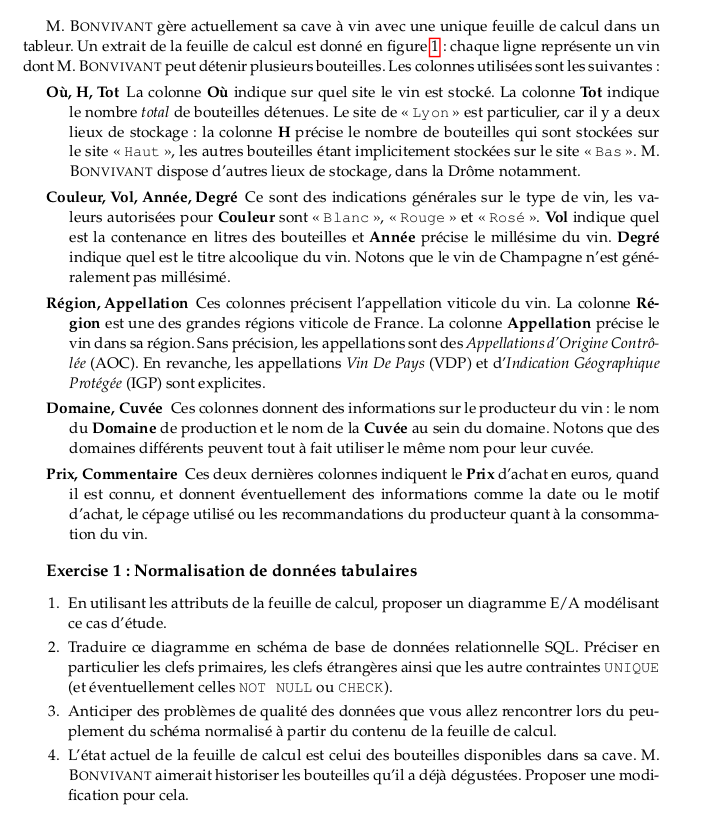
\includegraphics{images/tp_modelisation.png}
\caption{énoncé}
\end{figure}

\begin{figure}
\centering
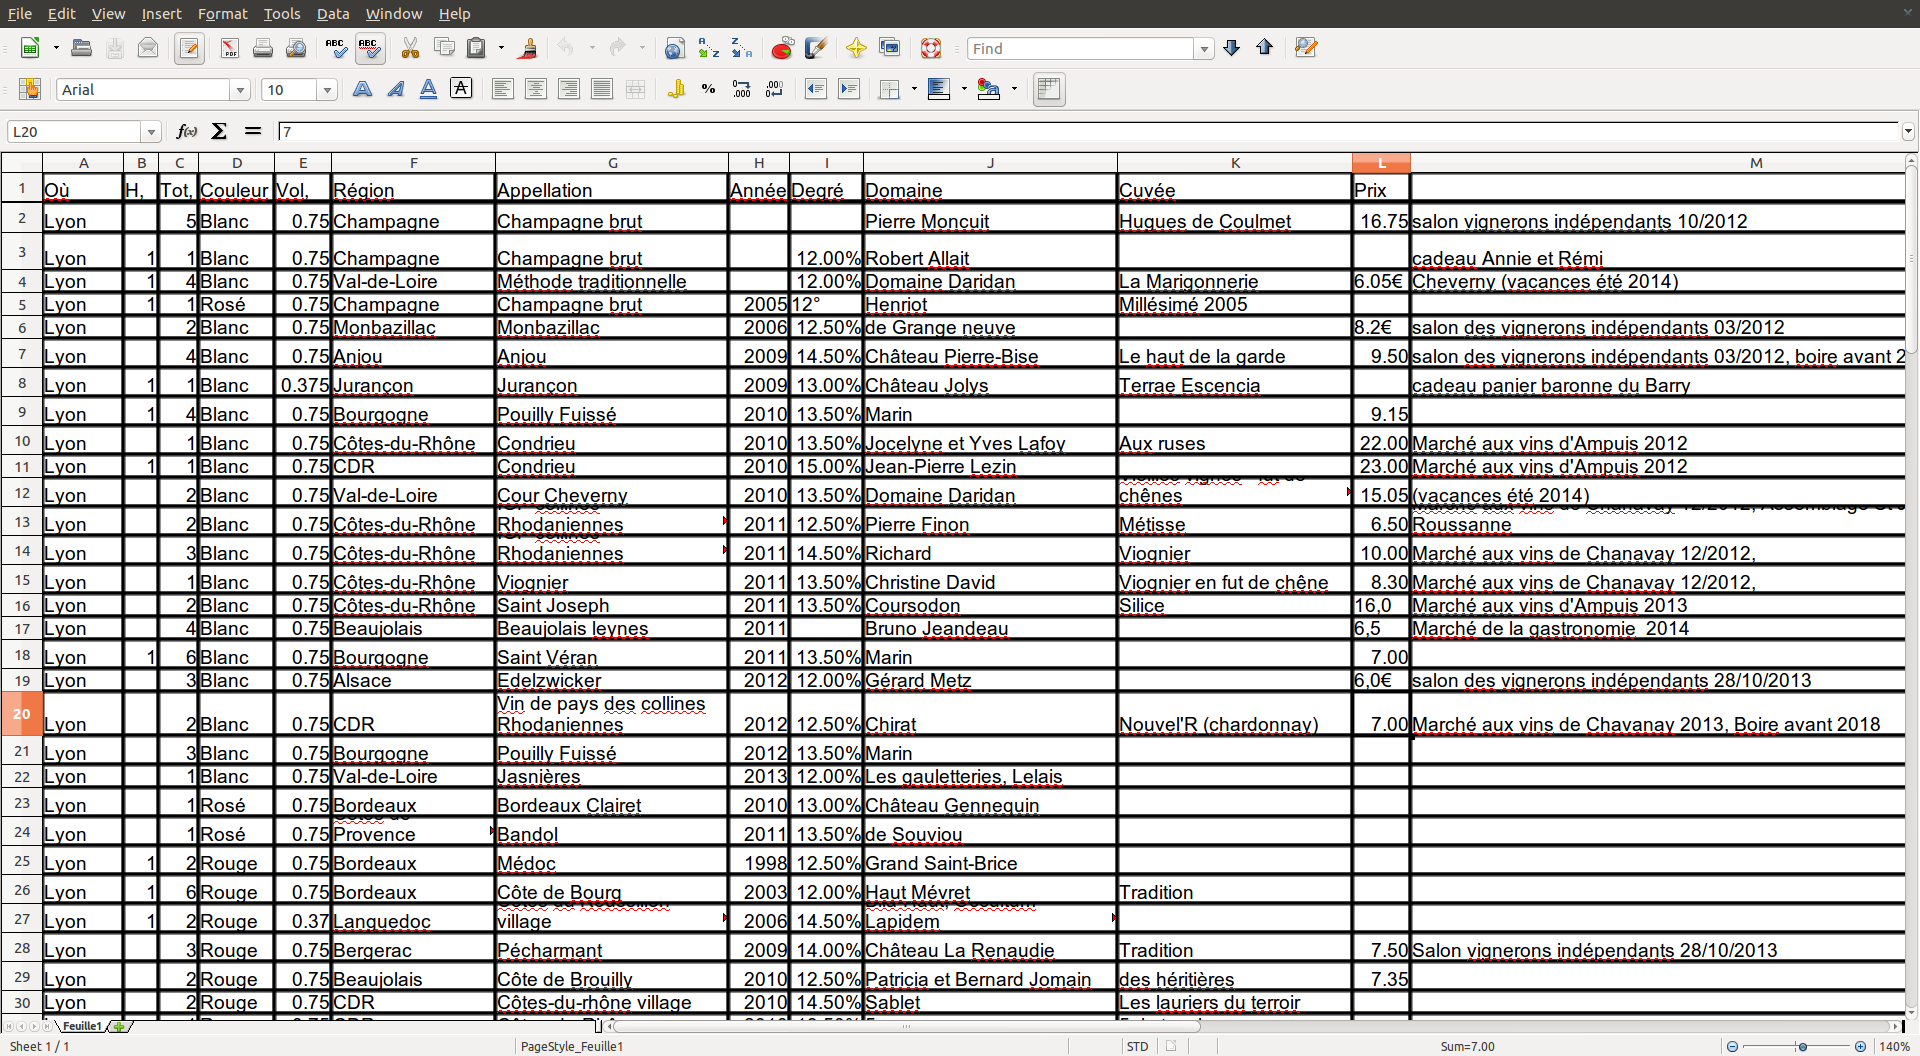
\includegraphics{images/tp_modelisation2.png}
\caption{énoncé}
\end{figure}

    \hypertarget{premier-diagramme-entituxe9sassociations-ruxe9alisuxe9-avec-mocodo}{%
\section{Premier Diagramme Entités/Associations réalisé avec
Mocodo}\label{premier-diagramme-entituxe9sassociations-ruxe9alisuxe9-avec-mocodo}}

\begin{figure}
\centering
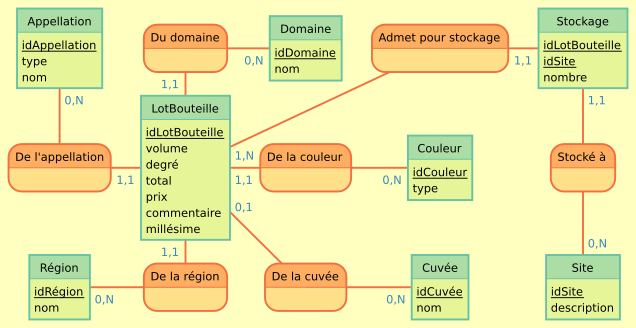
\includegraphics{mocodo/Lotbouteilles/Lotbouteilles.png}
\caption{diagramme E/A}
\end{figure}

    \hypertarget{schuxe9ma-sql-proposuxe9-par-mocodo}{%
\subsection{Schéma SQL proposé par
Mocodo}\label{schuxe9ma-sql-proposuxe9-par-mocodo}}

\begin{Shaded}
\begin{Highlighting}[]
\KeywordTok{CREATE} \KeywordTok{TABLE} \OtherTok{"APPELLATION"}\NormalTok{ (}
  \OtherTok{"idappellation"} \DataTypeTok{VARCHAR}\NormalTok{(}\DecValTok{42}\NormalTok{),}
  \OtherTok{"type"} \DataTypeTok{VARCHAR}\NormalTok{(}\DecValTok{42}\NormalTok{),}
  \OtherTok{"nom"} \DataTypeTok{VARCHAR}\NormalTok{(}\DecValTok{42}\NormalTok{),}
  \KeywordTok{PRIMARY} \KeywordTok{KEY}\NormalTok{ (}\OtherTok{"idappellation"}\NormalTok{)}
\NormalTok{);}

\KeywordTok{CREATE} \KeywordTok{TABLE} \OtherTok{"DOMAINE"}\NormalTok{ (}
  \OtherTok{"iddomaine"} \DataTypeTok{VARCHAR}\NormalTok{(}\DecValTok{42}\NormalTok{),}
  \OtherTok{"nom"} \DataTypeTok{VARCHAR}\NormalTok{(}\DecValTok{42}\NormalTok{),}
  \KeywordTok{PRIMARY} \KeywordTok{KEY}\NormalTok{ (}\OtherTok{"iddomaine"}\NormalTok{)}
\NormalTok{);}

\KeywordTok{CREATE} \KeywordTok{TABLE} \OtherTok{"STOCKAGE"}\NormalTok{ (}
  \OtherTok{"idlotbouteille"} \DataTypeTok{VARCHAR}\NormalTok{(}\DecValTok{42}\NormalTok{),}
  \OtherTok{"idsite"} \DataTypeTok{VARCHAR}\NormalTok{(}\DecValTok{42}\NormalTok{),}
  \OtherTok{"nombre"} \DataTypeTok{VARCHAR}\NormalTok{(}\DecValTok{42}\NormalTok{),}
  \OtherTok{"idlotbouteille\_1"} \DataTypeTok{VARCHAR}\NormalTok{(}\DecValTok{42}\NormalTok{),}
  \OtherTok{"idsite\_1"} \DataTypeTok{VARCHAR}\NormalTok{(}\DecValTok{42}\NormalTok{),}
  \KeywordTok{PRIMARY} \KeywordTok{KEY}\NormalTok{ (}\OtherTok{"idlotbouteille"}\NormalTok{, }\OtherTok{"idsite"}\NormalTok{),}
  \KeywordTok{FOREIGN} \KeywordTok{KEY}\NormalTok{ (}\OtherTok{"idlotbouteille\_1"}\NormalTok{) }\KeywordTok{REFERENCES} \OtherTok{"LOTBOUTEILLE"}\NormalTok{ (}\OtherTok{"idlotbouteille"}\NormalTok{),}
  \KeywordTok{FOREIGN} \KeywordTok{KEY}\NormalTok{ (}\OtherTok{"idsite\_1"}\NormalTok{) }\KeywordTok{REFERENCES} \OtherTok{"SITE"}\NormalTok{ (}\OtherTok{"idsite"}\NormalTok{)}
\NormalTok{);}

\KeywordTok{CREATE} \KeywordTok{TABLE} \OtherTok{"LOTBOUTEILLE"}\NormalTok{ (}
  \OtherTok{"idlotbouteille"} \DataTypeTok{VARCHAR}\NormalTok{(}\DecValTok{42}\NormalTok{),}
  \OtherTok{"volume"} \DataTypeTok{VARCHAR}\NormalTok{(}\DecValTok{42}\NormalTok{),}
  \OtherTok{"degré"} \DataTypeTok{VARCHAR}\NormalTok{(}\DecValTok{42}\NormalTok{),}
  \OtherTok{"total"} \DataTypeTok{VARCHAR}\NormalTok{(}\DecValTok{42}\NormalTok{),}
  \OtherTok{"prix"} \DataTypeTok{VARCHAR}\NormalTok{(}\DecValTok{42}\NormalTok{),}
  \OtherTok{"commentaire"} \DataTypeTok{VARCHAR}\NormalTok{(}\DecValTok{42}\NormalTok{),}
  \OtherTok{"millésime"} \DataTypeTok{VARCHAR}\NormalTok{(}\DecValTok{42}\NormalTok{),}
  \OtherTok{"idrégion"} \DataTypeTok{VARCHAR}\NormalTok{(}\DecValTok{42}\NormalTok{),}
  \OtherTok{"idappellation"} \DataTypeTok{VARCHAR}\NormalTok{(}\DecValTok{42}\NormalTok{),}
  \OtherTok{"idcuvée"} \DataTypeTok{VARCHAR}\NormalTok{(}\DecValTok{42}\NormalTok{),}
  \OtherTok{"iddomaine"} \DataTypeTok{VARCHAR}\NormalTok{(}\DecValTok{42}\NormalTok{),}
  \OtherTok{"idcouleur"} \DataTypeTok{VARCHAR}\NormalTok{(}\DecValTok{42}\NormalTok{),}
  \KeywordTok{PRIMARY} \KeywordTok{KEY}\NormalTok{ (}\OtherTok{"idlotbouteille"}\NormalTok{),}
  \KeywordTok{FOREIGN} \KeywordTok{KEY}\NormalTok{ (}\OtherTok{"idrégion"}\NormalTok{) }\KeywordTok{REFERENCES} \OtherTok{"RÉGION"}\NormalTok{ (}\OtherTok{"idrégion"}\NormalTok{),}
  \KeywordTok{FOREIGN} \KeywordTok{KEY}\NormalTok{ (}\OtherTok{"idappellation"}\NormalTok{) }\KeywordTok{REFERENCES} \OtherTok{"APPELLATION"}\NormalTok{ (}\OtherTok{"idappellation"}\NormalTok{),}
  \KeywordTok{FOREIGN} \KeywordTok{KEY}\NormalTok{ (}\OtherTok{"idcuvée"}\NormalTok{) }\KeywordTok{REFERENCES} \OtherTok{"CUVÉE"}\NormalTok{ (}\OtherTok{"idcuvée"}\NormalTok{),}
  \KeywordTok{FOREIGN} \KeywordTok{KEY}\NormalTok{ (}\OtherTok{"iddomaine"}\NormalTok{) }\KeywordTok{REFERENCES} \OtherTok{"DOMAINE"}\NormalTok{ (}\OtherTok{"iddomaine"}\NormalTok{),}
  \KeywordTok{FOREIGN} \KeywordTok{KEY}\NormalTok{ (}\OtherTok{"idcouleur"}\NormalTok{) }\KeywordTok{REFERENCES} \OtherTok{"COULEUR"}\NormalTok{ (}\OtherTok{"idcouleur"}\NormalTok{)}
\NormalTok{);}

\KeywordTok{CREATE} \KeywordTok{TABLE} \OtherTok{"COULEUR"}\NormalTok{ (}
  \OtherTok{"idcouleur"} \DataTypeTok{VARCHAR}\NormalTok{(}\DecValTok{42}\NormalTok{),}
  \OtherTok{"type"} \DataTypeTok{VARCHAR}\NormalTok{(}\DecValTok{42}\NormalTok{),}
  \KeywordTok{PRIMARY} \KeywordTok{KEY}\NormalTok{ (}\OtherTok{"idcouleur"}\NormalTok{)}
\NormalTok{);}

\KeywordTok{CREATE} \KeywordTok{TABLE} \OtherTok{"RÉGION"}\NormalTok{ (}
  \OtherTok{"idrégion"} \DataTypeTok{VARCHAR}\NormalTok{(}\DecValTok{42}\NormalTok{),}
  \OtherTok{"nom"} \DataTypeTok{VARCHAR}\NormalTok{(}\DecValTok{42}\NormalTok{),}
  \KeywordTok{PRIMARY} \KeywordTok{KEY}\NormalTok{ (}\OtherTok{"idrégion"}\NormalTok{)}
\NormalTok{);}

\KeywordTok{CREATE} \KeywordTok{TABLE} \OtherTok{"CUVÉE"}\NormalTok{ (}
  \OtherTok{"idcuvée"} \DataTypeTok{VARCHAR}\NormalTok{(}\DecValTok{42}\NormalTok{),}
  \OtherTok{"nom"} \DataTypeTok{VARCHAR}\NormalTok{(}\DecValTok{42}\NormalTok{),}
  \KeywordTok{PRIMARY} \KeywordTok{KEY}\NormalTok{ (}\OtherTok{"idcuvée"}\NormalTok{)}
\NormalTok{);}

\KeywordTok{CREATE} \KeywordTok{TABLE} \OtherTok{"SITE"}\NormalTok{ (}
  \OtherTok{"idsite"} \DataTypeTok{VARCHAR}\NormalTok{(}\DecValTok{42}\NormalTok{),}
  \OtherTok{"description"} \DataTypeTok{VARCHAR}\NormalTok{(}\DecValTok{42}\NormalTok{),}
  \KeywordTok{PRIMARY} \KeywordTok{KEY}\NormalTok{ (}\OtherTok{"idsite"}\NormalTok{)}
\NormalTok{);}
\end{Highlighting}
\end{Shaded}

    \hypertarget{description-du-schuxe9ma-sql}{%
\subsection{Description du schéma
SQL}\label{description-du-schuxe9ma-sql}}

{Appellation} ( {idAppellation}, {type}, {nom} )

Le champ idAppellation constitue la clef primaire de la table. C'était
déjà un identifiant de l'entité Appellation.

Les champs type et nom étaient déjà de simples attributs de l'entité
Appellation.

{Domaine} ( {idDomaine}, {nom} )

Le champ idDomaine constitue la clef primaire de la table. C'était déjà
un identifiant de l'entité Domaine.

Le champ nom était déjà un simple attribut de l'entité Domaine.

{Stockage} ( {idLotBouteille}, {idSite}, {nombre}, {idLotBouteille.1},
{idSite.1} )

Les champs idLotBouteille et idSite constituent la clef primaire de la
table. C'était déjà des identifiants de l'entité Stockage.

Le champ nombre était déjà un simple attribut de l'entité Stockage.

Le champ idLotBouteille.1 est une clef étrangère. Il a migré à partir de
l'entité LotBouteille par l'association de dépendance fonctionnelle
Admet pour stockage en perdant son caractère identifiant.

Le champ idSite.1 est une clef étrangère. Il a migré à partir de
l'entité Site par l'association de dépendance fonctionnelle Stocké à en
perdant son caractère identifiant.

{LotBouteille} ( {idLotBouteille}, {volume}, {degré}, {total}, {prix},
{commentaire}, {millésime}, {idRégion}, {idAppellation}, {idCuvée},
{idDomaine}, {idCouleur} )

Le champ idLotBouteille constitue la clef primaire de la table. C'était
déjà un identifiant de l'entité LotBouteille.

Les champs volume, degré, total, prix, commentaire et millésime étaient
déjà de simples attributs de l'entité LotBouteille.

Le champ idRégion est une clef étrangère. Il a migré à partir de
l'entité Région par l'association de dépendance fonctionnelle De la
région en perdant son caractère identifiant.

Le champ idAppellation est une clef étrangère. Il a migré à partir de
l'entité Appellation par l'association de dépendance fonctionnelle De
l'appellation en perdant son caractère identifiant.

Le champ idCuvée est une clef étrangère. Il a migré à partir de l'entité
Cuvée par l'association de dépendance fonctionnelle De la cuvée en
perdant son caractère identifiant.

Le champ idDomaine est une clef étrangère. Il a migré à partir de
l'entité Domaine par l'association de dépendance fonctionnelle Du
domaine en perdant son caractère identifiant.

Le champ idCouleur est une clef étrangère. Il a migré à partir de
l'entité Couleur par l'association de dépendance fonctionnelle De la
couleur en perdant son caractère identifiant.

{Couleur} ( {idCouleur}, {type} )

Le champ idCouleur constitue la clef primaire de la table. C'était déjà
un identifiant de l'entité Couleur.

Le champ type était déjà un simple attribut de l'entité Couleur.

{Région} ( {idRégion}, {nom} )

Le champ idRégion constitue la clef primaire de la table. C'était déjà
un identifiant de l'entité Région.

Le champ nom était déjà un simple attribut de l'entité Région.

{Cuvée} ( {idCuvée}, {nom} )

Le champ idCuvée constitue la clef primaire de la table. C'était déjà un
identifiant de l'entité Cuvée.

Le champ nom était déjà un simple attribut de l'entité Cuvée.

{Site} ( {idSite}, {description} )

Le champ idSite constitue la clef primaire de la table. C'était déjà un
identifiant de l'entité Site.

Le champ description était déjà un simple attribut de l'entité Site.

    \hypertarget{affinement-du-schuxe9ma-sql-types-et-contraintes}{%
\subsection{Affinement du schéma SQL (types et
contraintes)}\label{affinement-du-schuxe9ma-sql-types-et-contraintes}}

\begin{Shaded}
\begin{Highlighting}[]
\KeywordTok{CREATE} \KeywordTok{TABLE} \OtherTok{"APPELLATION"}\NormalTok{ (}
  \OtherTok{"idappellation"} \DataTypeTok{INTEGER} \KeywordTok{NOT} \KeywordTok{NULL} \KeywordTok{PRIMARY} \KeywordTok{KEY}\NormalTok{,}
  \OtherTok{"type"} \DataTypeTok{VARCHAR}\NormalTok{(}\DecValTok{42}\NormalTok{) }\KeywordTok{CHECK}\NormalTok{( }\OtherTok{"type"} \KeywordTok{IN}\NormalTok{ (}\OtherTok{"AOC"}\NormalTok{, }\OtherTok{"VDP"}\NormalTok{, }\OtherTok{"IGP"}\NormalTok{)), }\CommentTok{{-}{-}NULL représenterait AOC}
  \OtherTok{"nom"} \DataTypeTok{VARCHAR}\NormalTok{(}\DecValTok{42}\NormalTok{) }\KeywordTok{NOT} \KeywordTok{NULL}
\NormalTok{);}

\KeywordTok{CREATE} \KeywordTok{TABLE} \OtherTok{"DOMAINE"}\NormalTok{ (}
  \OtherTok{"iddomaine"} \DataTypeTok{INTEGER} \KeywordTok{NOT} \KeywordTok{NULL} \KeywordTok{PRIMARY} \KeywordTok{KEY}\NormalTok{,}
  \OtherTok{"nom"} \DataTypeTok{VARCHAR}\NormalTok{(}\DecValTok{42}\NormalTok{)  }\KeywordTok{NOT} \KeywordTok{NULL} \KeywordTok{UNIQUE}         \CommentTok{{-}{-} un nom de domaine est unique                        }
\NormalTok{);}

\KeywordTok{CREATE} \KeywordTok{TABLE} \OtherTok{"STOCKAGE"}\NormalTok{ (}
  \OtherTok{"idlotbouteille"} \DataTypeTok{INTEGER} \KeywordTok{NOT} \KeywordTok{NULL}
  \OtherTok{"idsite"} \DataTypeTok{INTEGER} \KeywordTok{NOT} \KeywordTok{NULL}\NormalTok{,}
  \OtherTok{"nombre"} \DataTypeTok{INTEGER} \KeywordTok{NOT} \KeywordTok{NULL}\NormalTok{,}
  \KeywordTok{PRIMARY} \KeywordTok{KEY}\NormalTok{ (}\OtherTok{"idlotbouteille"}\NormalTok{, }\OtherTok{"idsite"}\NormalTok{),}
  \KeywordTok{FOREIGN} \KeywordTok{KEY}\NormalTok{ (}\OtherTok{"idlotbouteille"}\NormalTok{) }\KeywordTok{REFERENCES} \OtherTok{"LOTBOUTEILLE"}\NormalTok{ (}\OtherTok{"idlotbouteille"}\NormalTok{),}
  \KeywordTok{FOREIGN} \KeywordTok{KEY}\NormalTok{ (}\OtherTok{"idsite"}\NormalTok{) }\KeywordTok{REFERENCES} \OtherTok{"SITE"}\NormalTok{ (}\OtherTok{"idsite"}\NormalTok{)}
\NormalTok{);}

\KeywordTok{CREATE} \KeywordTok{TABLE} \OtherTok{"LOTBOUTEILLE"}\NormalTok{ (}
  \OtherTok{"idlotbouteille"} \DataTypeTok{INTEGER} \KeywordTok{NOT} \KeywordTok{NULL} \KeywordTok{PRIMARY} \KeywordTok{KEY}\NormalTok{,}
  \OtherTok{"volume"} \DataTypeTok{REAL} \KeywordTok{NOT} \KeywordTok{NULL} \KeywordTok{CHECK}\NormalTok{(volume }\OperatorTok{>=} \DecValTok{0}\NormalTok{),}
  \OtherTok{"degré"} \DataTypeTok{REAL} \KeywordTok{NOT} \KeywordTok{NULL} \KeywordTok{CHECK}\NormalTok{(degré }\OperatorTok{>=} \DecValTok{0}\NormalTok{),}
  \OtherTok{"total"} \DataTypeTok{INTEGER} \KeywordTok{NOT} \KeywordTok{NULL} \KeywordTok{CHECK}\NormalTok{(total }\OperatorTok{>=} \DecValTok{0}\NormalTok{),}
  \OtherTok{"prix"} \DataTypeTok{REAL} \KeywordTok{NOT} \KeywordTok{NULL} \KeywordTok{CHECK}\NormalTok{(prix }\OperatorTok{>=} \DecValTok{0}\NormalTok{),}
  \OtherTok{"commentaire"} \DataTypeTok{VARCHAR}\NormalTok{(}\DecValTok{42}\NormalTok{),}
  \OtherTok{"millésime"} \DataTypeTok{INTEGER} \KeywordTok{CHECK}\NormalTok{(millésime }\OperatorTok{>=} \DecValTok{0}\NormalTok{),}
  \OtherTok{"idrégion"} \DataTypeTok{INTEGER} \KeywordTok{NOT} \KeywordTok{NULL}\NormalTok{,}
  \OtherTok{"idappellation"} \DataTypeTok{INTEGER} \KeywordTok{NOT} \KeywordTok{NULL}\NormalTok{,}
  \OtherTok{"idcuvée"} \DataTypeTok{INTEGER} \KeywordTok{NOT} \KeywordTok{NULL}\NormalTok{,}
  \OtherTok{"iddomaine"} \DataTypeTok{INTEGER} \KeywordTok{NOT} \KeywordTok{NULL}\NormalTok{,}
  \OtherTok{"idcouleur"} \DataTypeTok{INTEGER} \KeywordTok{NOT} \KeywordTok{NULL}\NormalTok{,}
  \KeywordTok{PRIMARY} \KeywordTok{KEY}\NormalTok{ (}\OtherTok{"idlotbouteille"}\NormalTok{),}
  \KeywordTok{FOREIGN} \KeywordTok{KEY}\NormalTok{ (}\OtherTok{"idrégion"}\NormalTok{) }\KeywordTok{REFERENCES} \OtherTok{"RÉGION"}\NormalTok{ (}\OtherTok{"idrégion"}\NormalTok{),}
  \KeywordTok{FOREIGN} \KeywordTok{KEY}\NormalTok{ (}\OtherTok{"idappellation"}\NormalTok{) }\KeywordTok{REFERENCES} \OtherTok{"APPELLATION"}\NormalTok{ (}\OtherTok{"idappellation"}\NormalTok{),}
  \KeywordTok{FOREIGN} \KeywordTok{KEY}\NormalTok{ (}\OtherTok{"idcuvée"}\NormalTok{) }\KeywordTok{REFERENCES} \OtherTok{"CUVÉE"}\NormalTok{ (}\OtherTok{"idcuvée"}\NormalTok{),}
  \KeywordTok{FOREIGN} \KeywordTok{KEY}\NormalTok{ (}\OtherTok{"iddomaine"}\NormalTok{) }\KeywordTok{REFERENCES} \OtherTok{"DOMAINE"}\NormalTok{ (}\OtherTok{"iddomaine"}\NormalTok{),}
  \KeywordTok{FOREIGN} \KeywordTok{KEY}\NormalTok{ (}\OtherTok{"idcouleur"}\NormalTok{) }\KeywordTok{REFERENCES} \OtherTok{"COULEUR"}\NormalTok{ (}\OtherTok{"idcouleur"}\NormalTok{)}
\NormalTok{);}

\KeywordTok{CREATE} \KeywordTok{TABLE} \OtherTok{"COULEUR"}\NormalTok{ (}
  \OtherTok{"idcouleur"} \DataTypeTok{INTEGER} \KeywordTok{NOT} \KeywordTok{NULL} \KeywordTok{PRIMARY} \KeywordTok{KEY}\NormalTok{,}
  \OtherTok{"type"} \DataTypeTok{VARCHAR}\NormalTok{(}\DecValTok{42}\NormalTok{)}\KeywordTok{NOT} \KeywordTok{NULL}  \KeywordTok{UNIQUE}
\NormalTok{);}

\KeywordTok{CREATE} \KeywordTok{TABLE} \OtherTok{"RÉGION"}\NormalTok{ (}
  \OtherTok{"idrégion"}  \DataTypeTok{INTEGER} \KeywordTok{NOT} \KeywordTok{NULL} \KeywordTok{PRIMARY} \KeywordTok{KEY}\NormalTok{,}
  \OtherTok{"nom"} \KeywordTok{NOT} \KeywordTok{NULL}  \KeywordTok{UNIQUE}
\NormalTok{);}

\KeywordTok{CREATE} \KeywordTok{TABLE} \OtherTok{"CUVÉE"}\NormalTok{ (}
  \OtherTok{"idcuvée"}  \DataTypeTok{INTEGER} \KeywordTok{NOT} \KeywordTok{NULL} \KeywordTok{PRIMARY} \KeywordTok{KEY}\NormalTok{,}
  \OtherTok{"nom"} \DataTypeTok{VARCHAR}\NormalTok{(}\DecValTok{42}\NormalTok{) }\KeywordTok{NOT} \KeywordTok{NULL}  \KeywordTok{UNIQUE}                \CommentTok{{-}{-}un nom de cuvée est unique}
\NormalTok{);}

\KeywordTok{CREATE} \KeywordTok{TABLE} \OtherTok{"SITE"}\NormalTok{ (}
  \OtherTok{"idsite"} \DataTypeTok{INTEGER} \KeywordTok{NOT} \KeywordTok{NULL} \KeywordTok{PRIMARY} \KeywordTok{KEY}\NormalTok{,}
  \OtherTok{"description"} \DataTypeTok{VARCHAR}\NormalTok{(}\DecValTok{42}\NormalTok{) }\KeywordTok{NOT} \KeywordTok{NULL} \KeywordTok{UNIQUE}  
\NormalTok{);}
\end{Highlighting}
\end{Shaded}

    \hypertarget{second-diagramme-entituxe9sassociations-ruxe9alisuxe9-avec-mocodo}{%
\subsection{Second Diagramme Entités/Associations réalisé avec
Mocodo}\label{second-diagramme-entituxe9sassociations-ruxe9alisuxe9-avec-mocodo}}

\begin{figure}
\centering
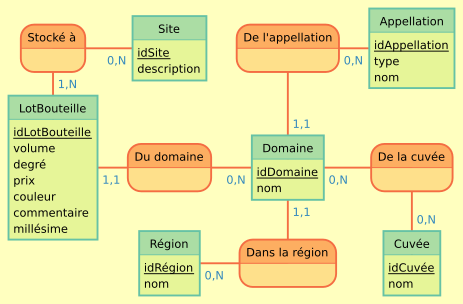
\includegraphics{mocodo/Domaines/Domaines.png}
\caption{diagramme E/A}
\end{figure}

    {Stocké à} ( {idLotBouteille}, {idSite} )

Le champ idLotBouteille fait partie de la clef primaire de la table.
C'est une clef étrangère qui a migré directement à partir de l'entité
LotBouteille.

Le champ idSite fait partie de la clef primaire de la table. C'est une
clef étrangère qui a migré directement à partir de l'entité Site.

{Site} ( {idSite}, {description} )

Le champ idSite constitue la clef primaire de la table. C'était déjà un
identifiant de l'entité Site.

Le champ description était déjà un simple attribut de l'entité Site.

{Appellation} ( {idAppellation}, {type}, {nom} )

Le champ idAppellation constitue la clef primaire de la table. C'était
déjà un identifiant de l'entité Appellation.

Les champs type et nom étaient déjà de simples attributs de l'entité
Appellation.

{LotBouteille} ( {idLotBouteille}, {volume}, {degré}, {prix}, {couleur},
{commentaire}, {millésime}, {idDomaine} )

Le champ idLotBouteille constitue la clef primaire de la table. C'était
déjà un identifiant de l'entité LotBouteille.

Les champs volume, degré, prix, couleur, commentaire et millésime
étaient déjà de simples attributs de l'entité LotBouteille.

Le champ idDomaine est une clef étrangère. Il a migré à partir de
l'entité Domaine par l'association de dépendance fonctionnelle Du
domaine en perdant son caractère identifiant.

{Domaine} ( {idDomaine}, {nom}, {idAppellation}, {idRégion} )

Le champ idDomaine constitue la clef primaire de la table. C'était déjà
un identifiant de l'entité Domaine.

Le champ nom était déjà un simple attribut de l'entité Domaine.

Le champ idAppellation est une clef étrangère. Il a migré à partir de
l'entité Appellation par l'association de dépendance fonctionnelle De
l'appellation en perdant son caractère identifiant.

Le champ idRégion est une clef étrangère. Il a migré à partir de
l'entité Région par l'association de dépendance fonctionnelle Dans la
région en perdant son caractère identifiant.

{De la cuvée} ( {idDomaine}, {idCuvée} )

Le champ idDomaine fait partie de la clef primaire de la table. C'est
une clef étrangère qui a migré directement à partir de l'entité Domaine.

Le champ idCuvée fait partie de la clef primaire de la table. C'est une
clef étrangère qui a migré directement à partir de l'entité Cuvée.

{Région} ( {idRégion}, {nom} )

Le champ idRégion constitue la clef primaire de la table. C'était déjà
un identifiant de l'entité Région.

Le champ nom était déjà un simple attribut de l'entité Région.

{Cuvée} ( {idCuvée}, {nom} )

Le champ idCuvée constitue la clef primaire de la table. C'était déjà un
identifiant de l'entité Cuvée.

Le champ nom était déjà un simple attribut de l'entité Cuvée.

\hypertarget{schuxe9ma-sql-avec-contraintes}{%
\section{Schéma SQL avec
contraintes}\label{schuxe9ma-sql-avec-contraintes}}

\begin{Shaded}
\begin{Highlighting}[]
\KeywordTok{CREATE} \KeywordTok{TABLE} \OtherTok{"APPELLATION"}\NormalTok{ (}
  \OtherTok{"idappellation"} \DataTypeTok{INTEGER} \KeywordTok{NOT} \KeywordTok{NULL} \KeywordTok{PRIMARY} \KeywordTok{KEY}\NormalTok{,}
  \OtherTok{"type"} \DataTypeTok{VARCHAR}\NormalTok{(}\DecValTok{42}\NormalTok{) }\KeywordTok{CHECK}\NormalTok{( }\OtherTok{"type"} \KeywordTok{IN}\NormalTok{ (}\OtherTok{"AOC"}\NormalTok{, }\OtherTok{"VDP"}\NormalTok{, }\OtherTok{"IGP"}\NormalTok{)), }\CommentTok{{-}{-}NULL représenterait AOC}
  \OtherTok{"nom"} \DataTypeTok{VARCHAR}\NormalTok{(}\DecValTok{42}\NormalTok{) }\KeywordTok{NOT} \KeywordTok{NULL}
\NormalTok{);}




\KeywordTok{CREATE} \KeywordTok{TABLE} \OtherTok{"STOCKAGE"}\NormalTok{ (}
  \OtherTok{"idlotbouteille"} \DataTypeTok{INTEGER} \KeywordTok{NOT} \KeywordTok{NULL}\NormalTok{,}
  \OtherTok{"idsite"} \DataTypeTok{INTEGER} \KeywordTok{NOT} \KeywordTok{NULL}\NormalTok{,}
  \OtherTok{"nombre"} \DataTypeTok{INTEGER} \KeywordTok{NOT} \KeywordTok{NULL} \KeywordTok{CHECK}\NormalTok{(nombre }\OperatorTok{>=} \DecValTok{0}\NormalTok{),}
  \KeywordTok{PRIMARY} \KeywordTok{KEY}\NormalTok{ (}\OtherTok{"idlotbouteille"}\NormalTok{, }\OtherTok{"idsite"}\NormalTok{),}
  \KeywordTok{FOREIGN} \KeywordTok{KEY}\NormalTok{ (}\OtherTok{"idlotbouteille"}\NormalTok{) }\KeywordTok{REFERENCES} \OtherTok{"LOTBOUTEILLE"}\NormalTok{ (}\OtherTok{"idlotbouteille"}\NormalTok{),}
  \KeywordTok{FOREIGN} \KeywordTok{KEY}\NormalTok{ (}\OtherTok{"idsite"}\NormalTok{) }\KeywordTok{REFERENCES} \OtherTok{"SITE"}\NormalTok{ (}\OtherTok{"idsite"}\NormalTok{)}
\NormalTok{);}




\KeywordTok{CREATE} \KeywordTok{TABLE} \OtherTok{"DOMAINE"}\NormalTok{ (}
   \OtherTok{"iddomaine"} \DataTypeTok{INTEGER} \KeywordTok{NOT} \KeywordTok{NULL} \KeywordTok{PRIMARY} \KeywordTok{KEY}\NormalTok{,}
    \OtherTok{"nom"} \DataTypeTok{VARCHAR}\NormalTok{(}\DecValTok{42}\NormalTok{)  }\KeywordTok{NOT} \KeywordTok{NULL}\NormalTok{,       }\CommentTok{{-}{-} un nom de domaine n\textquotesingle{}est pas forcément unique (des domaines de même nom dans des régions différentes)  }
  \OtherTok{"idrégion"} \DataTypeTok{INTEGER} \KeywordTok{NOT} \KeywordTok{NULL}\NormalTok{,}
  \OtherTok{"idcuvée"} \DataTypeTok{INTEGER} \KeywordTok{NOT} \KeywordTok{NULL}\NormalTok{,}
  \OtherTok{"idappellation"} \DataTypeTok{INTEGER} \KeywordTok{NOT} \KeywordTok{NULL}\NormalTok{,}
  \KeywordTok{FOREIGN} \KeywordTok{KEY}\NormalTok{ (}\OtherTok{"idappellation"}\NormalTok{) }\KeywordTok{REFERENCES} \OtherTok{"APPELLATION"}\NormalTok{ (}\OtherTok{"idappellation"}\NormalTok{),}
  \KeywordTok{FOREIGN} \KeywordTok{KEY}\NormalTok{ (}\OtherTok{"idcuvée"}\NormalTok{) }\KeywordTok{REFERENCES} \OtherTok{"CUVÉE"}\NormalTok{ (}\OtherTok{"idcuvée"}\NormalTok{),}
  \KeywordTok{FOREIGN} \KeywordTok{KEY}\NormalTok{ (}\OtherTok{"idrégion"}\NormalTok{) }\KeywordTok{REFERENCES} \OtherTok{"RÉGION"}\NormalTok{ (}\OtherTok{"idrégion"}\NormalTok{)}
\NormalTok{);}


\KeywordTok{CREATE} \KeywordTok{TABLE} \OtherTok{"LOTBOUTEILLE"}\NormalTok{ (}
  \OtherTok{"idlotbouteille"} \DataTypeTok{INTEGER} \KeywordTok{NOT} \KeywordTok{NULL} \KeywordTok{PRIMARY} \KeywordTok{KEY}\NormalTok{,}
  \OtherTok{"volume"} \DataTypeTok{REAL} \KeywordTok{NOT} \KeywordTok{NULL} \KeywordTok{CHECK}\NormalTok{(volume }\OperatorTok{>=} \DecValTok{0}\NormalTok{),}
  \OtherTok{"degré"} \DataTypeTok{REAL} \KeywordTok{NOT} \KeywordTok{NULL} \KeywordTok{CHECK}\NormalTok{(degré }\OperatorTok{>=} \DecValTok{0}\NormalTok{),}
  \OtherTok{"prix"} \DataTypeTok{REAL} \KeywordTok{NOT} \KeywordTok{NULL} \KeywordTok{CHECK}\NormalTok{(prix }\OperatorTok{>=} \DecValTok{0}\NormalTok{),}
  \OtherTok{"commentaire"} \DataTypeTok{VARCHAR}\NormalTok{(}\DecValTok{42}\NormalTok{),  }\CommentTok{{-}{-}peut être NULL}
  \OtherTok{"millésime"} \DataTypeTok{INTEGER} \KeywordTok{CHECK}\NormalTok{(millésime }\OperatorTok{>=} \DecValTok{0}\NormalTok{),}
  \OtherTok{"couleur"} \DataTypeTok{VARCHAR}\NormalTok{(}\DecValTok{42}\NormalTok{) }\KeywordTok{NOT} \KeywordTok{NULL} \KeywordTok{CHECK}\NormalTok{(}\FunctionTok{lower}\NormalTok{(couleur) }\KeywordTok{in}\NormalTok{ (}\OtherTok{"blanc"}\NormalTok{, }\OtherTok{"rosé"}\NormalTok{, }\OtherTok{"rouge"}\NormalTok{)),}
  \OtherTok{"iddomaine"} \DataTypeTok{INTEGER} \KeywordTok{NOT} \KeywordTok{NULL}\NormalTok{,}
  \KeywordTok{FOREIGN} \KeywordTok{KEY}\NormalTok{ (}\OtherTok{"iddomaine"}\NormalTok{) }\KeywordTok{REFERENCES} \OtherTok{"DOMAINE"}\NormalTok{ (}\OtherTok{"iddomaine"}\NormalTok{)}
\NormalTok{);}


\KeywordTok{CREATE} \KeywordTok{TABLE} \OtherTok{"RÉGION"}\NormalTok{ (}
  \OtherTok{"idrégion"}  \DataTypeTok{INTEGER} \KeywordTok{NOT} \KeywordTok{NULL} \KeywordTok{PRIMARY} \KeywordTok{KEY}\NormalTok{,}
  \OtherTok{"nom"} \KeywordTok{NOT} \KeywordTok{NULL}  \KeywordTok{UNIQUE}
\NormalTok{);}

\KeywordTok{CREATE} \KeywordTok{TABLE} \OtherTok{"CUVÉE"}\NormalTok{ (}
  \OtherTok{"idcuvée"}  \DataTypeTok{INTEGER} \KeywordTok{NOT} \KeywordTok{NULL} \KeywordTok{PRIMARY} \KeywordTok{KEY}\NormalTok{,}
  \OtherTok{"nom"} \DataTypeTok{VARCHAR}\NormalTok{(}\DecValTok{42}\NormalTok{)   }\KeywordTok{UNIQUE}                \CommentTok{{-}{-}un nom de cuvée est unique mais peut être vide}
\NormalTok{);}

\KeywordTok{CREATE} \KeywordTok{TABLE} \OtherTok{"SITE"}\NormalTok{ (}
  \OtherTok{"idsite"} \DataTypeTok{INTEGER} \KeywordTok{NOT} \KeywordTok{NULL} \KeywordTok{PRIMARY} \KeywordTok{KEY}\NormalTok{,}
  \OtherTok{"description"} \DataTypeTok{VARCHAR}\NormalTok{(}\DecValTok{42}\NormalTok{) }\KeywordTok{NOT} \KeywordTok{NULL} \KeywordTok{UNIQUE}  
\NormalTok{);}


\KeywordTok{CREATE} \KeywordTok{TABLE} \OtherTok{"DE\_LA\_CUVÉE"}\NormalTok{ (}
  \OtherTok{"iddomaine"} \DataTypeTok{VARCHAR}\NormalTok{(}\DecValTok{42}\NormalTok{),}
  \OtherTok{"idcuvée"} \DataTypeTok{VARCHAR}\NormalTok{(}\DecValTok{42}\NormalTok{),}
  \KeywordTok{PRIMARY} \KeywordTok{KEY}\NormalTok{ (}\OtherTok{"iddomaine"}\NormalTok{, }\OtherTok{"idcuvée"}\NormalTok{),}
  \KeywordTok{FOREIGN} \KeywordTok{KEY}\NormalTok{ (}\OtherTok{"iddomaine"}\NormalTok{) }\KeywordTok{REFERENCES} \OtherTok{"DOMAINE"}\NormalTok{ (}\OtherTok{"iddomaine"}\NormalTok{),}
  \KeywordTok{FOREIGN} \KeywordTok{KEY}\NormalTok{ (}\OtherTok{"idcuvée"}\NormalTok{) }\KeywordTok{REFERENCES} \OtherTok{"CUVÉE"}\NormalTok{ (}\OtherTok{"idcuvée"}\NormalTok{)}
\NormalTok{);}
\end{Highlighting}
\end{Shaded}

    \begin{Verbatim}[commandchars=\\\{\}]
{\color{incolor}In [{\color{incolor}29}]:} \PY{o}{\PYZpc{}\PYZpc{}}\PY{k}{sql}
         
         CREATE TABLE \PYZdq{}APPELLATION\PYZdq{} (
           \PYZdq{}idappellation\PYZdq{} INTEGER NOT NULL PRIMARY KEY,
           \PYZdq{}type\PYZdq{} VARCHAR(42) CHECK( \PYZdq{}type\PYZdq{} IN (\PYZdq{}AOC\PYZdq{}, \PYZdq{}VDP\PYZdq{}, \PYZdq{}IGP\PYZdq{})), \PYZhy{}\PYZhy{}NULL représenterait AOC
           \PYZdq{}nom\PYZdq{} VARCHAR(42) NOT NULL
         );
         
         
         
         CREATE TABLE \PYZdq{}STOCKAGE\PYZdq{} (
           \PYZdq{}idlotbouteille\PYZdq{} INTEGER NOT NULL,
           \PYZdq{}idsite\PYZdq{} INTEGER NOT NULL,
           \PYZdq{}nombre\PYZdq{} INTEGER NOT NULL CHECK(nombre \PYZgt{}= 0),
           PRIMARY KEY (\PYZdq{}idlotbouteille\PYZdq{}, \PYZdq{}idsite\PYZdq{}),
           FOREIGN KEY (\PYZdq{}idlotbouteille\PYZdq{}) REFERENCES \PYZdq{}LOTBOUTEILLE\PYZdq{} (\PYZdq{}idlotbouteille\PYZdq{}),
           FOREIGN KEY (\PYZdq{}idsite\PYZdq{}) REFERENCES \PYZdq{}SITE\PYZdq{} (\PYZdq{}idsite\PYZdq{})
         );
         
         
         
         
         CREATE TABLE \PYZdq{}DOMAINE\PYZdq{} (
            \PYZdq{}iddomaine\PYZdq{} INTEGER NOT NULL PRIMARY KEY,
             \PYZdq{}nom\PYZdq{} VARCHAR(42)  NOT NULL,       \PYZhy{}\PYZhy{} un nom de domaine n\PYZsq{}est pas forcément unique (des domaines de même nom dans des régions différentes)  
           \PYZdq{}idrégion\PYZdq{} INTEGER NOT NULL,
           \PYZdq{}idcuvée\PYZdq{} INTEGER NOT NULL,
           \PYZdq{}idappellation\PYZdq{} INTEGER NOT NULL,
           FOREIGN KEY (\PYZdq{}idappellation\PYZdq{}) REFERENCES \PYZdq{}APPELLATION\PYZdq{} (\PYZdq{}idappellation\PYZdq{}),
           FOREIGN KEY (\PYZdq{}idcuvée\PYZdq{}) REFERENCES \PYZdq{}CUVÉE\PYZdq{} (\PYZdq{}idcuvée\PYZdq{}),
           FOREIGN KEY (\PYZdq{}idrégion\PYZdq{}) REFERENCES \PYZdq{}RÉGION\PYZdq{} (\PYZdq{}idrégion\PYZdq{})
         );
         
         
         CREATE TABLE \PYZdq{}LOTBOUTEILLE\PYZdq{} (
           \PYZdq{}idlotbouteille\PYZdq{} INTEGER NOT NULL PRIMARY KEY,
           \PYZdq{}volume\PYZdq{} REAL NOT NULL CHECK(volume \PYZgt{}= 0),
           \PYZdq{}degré\PYZdq{} REAL  CHECK(degré \PYZgt{}= 0),
           \PYZdq{}prix\PYZdq{} REAL  CHECK(prix \PYZgt{}= 0),
           \PYZdq{}commentaire\PYZdq{} TEXT,  \PYZhy{}\PYZhy{}peut être NULL
           \PYZdq{}millésime\PYZdq{} INTEGER CHECK(millésime \PYZgt{}= 0),
           \PYZdq{}couleur\PYZdq{} VARCHAR(5) NOT NULL CHECK(lower(couleur) in (\PYZdq{}blanc\PYZdq{}, \PYZdq{}rosé\PYZdq{}, \PYZdq{}rouge\PYZdq{})),
           \PYZdq{}iddomaine\PYZdq{} INTEGER NOT NULL,
           FOREIGN KEY (\PYZdq{}iddomaine\PYZdq{}) REFERENCES \PYZdq{}DOMAINE\PYZdq{} (\PYZdq{}iddomaine\PYZdq{})
         );
         
         
         CREATE TABLE \PYZdq{}RÉGION\PYZdq{} (
           \PYZdq{}idrégion\PYZdq{}  INTEGER NOT NULL PRIMARY KEY,
           \PYZdq{}nom\PYZdq{} NOT NULL  UNIQUE
         );
         
         CREATE TABLE \PYZdq{}CUVÉE\PYZdq{} (
           \PYZdq{}idcuvée\PYZdq{}  INTEGER NOT NULL PRIMARY KEY,
           \PYZdq{}nom\PYZdq{} VARCHAR(42)   UNIQUE                \PYZhy{}\PYZhy{}un nom de cuvée est unique mais peut être vide
         );
         
         CREATE TABLE \PYZdq{}SITE\PYZdq{} (
           \PYZdq{}idsite\PYZdq{} INTEGER NOT NULL PRIMARY KEY,
           \PYZdq{}description\PYZdq{} VARCHAR(42) NOT NULL UNIQUE  
         );
\end{Verbatim}


    \begin{Verbatim}[commandchars=\\\{\}]
Done.
Done.
Done.
Done.
Done.
Done.
Done.

    \end{Verbatim}

\begin{Verbatim}[commandchars=\\\{\}]
{\color{outcolor}Out[{\color{outcolor}29}]:} []
\end{Verbatim}
            
    \hypertarget{probluxe8mes-de-qualituxe9-des-donnuxe9es-que-nous-risquons-de-rencontrer-lors-du-peuplement-de-la-table}{%
\subsection{Problèmes de qualité des données que nous risquons de
rencontrer lors du peuplement de la
table}\label{probluxe8mes-de-qualituxe9-des-donnuxe9es-que-nous-risquons-de-rencontrer-lors-du-peuplement-de-la-table}}

\begin{itemize}
\tightlist
\item
  Le deuxième schéma propose un meilleur découpage des données entre
  stockage, lot de bouteille et terroir (domaine, région, appellation)
\item
  Un même lot de bouteilles peut être stocké dans plusieurs sites grace
  à la table stockage : on distinguera par exemple dans la table site
  les deux sites de stockage sur Lyon. On a supprimé l'attribut total
  pour un lot de bouteilles, on peut le retrouver en faisant la somme
  des nombres de bouteilles de tous les stockages associés à un lot.
\item
  avec ce modèle on ne peut pas distinguer des achats du même millés
\item
  Les orthographes de certains attibuts (régions, appellations) sont
  variables
\item
  Les formats des titrages en degrés sont variables
\item
\end{itemize}

    \hypertarget{rajout-dun-table-duxe9gustation-pour-historiser-les-duxe9gustations}{%
\subsection{Rajout d'un table Dégustation pour historiser les
dégustations}\label{rajout-dun-table-duxe9gustation-pour-historiser-les-duxe9gustations}}

\begin{figure}
\centering
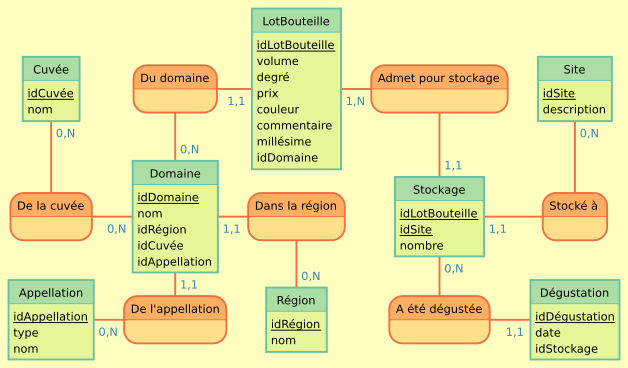
\includegraphics{mocodo/Stockages/Stockages.png}
\caption{diagramme E/A}
\end{figure}

{Site} ( {idSite}, {description} )

Le champ idSite constitue la clef primaire de la table. C'était déjà un
identifiant de l'entité Site.

Le champ description était déjà un simple attribut de l'entité Site.

{Région} ( {idRégion}, {nom} )

Le champ idRégion constitue la clef primaire de la table. C'était déjà
un identifiant de l'entité Région.

Le champ nom était déjà un simple attribut de l'entité Région.

{Cuvée} ( {idCuvée}, {nom} )

Le champ idCuvée constitue la clef primaire de la table. C'était déjà un
identifiant de l'entité Cuvée.

Le champ nom était déjà un simple attribut de l'entité Cuvée.

{Stockage} ( {idStockage}, {idLotBouteille}, {idSite}, {nombre},
{idLotBouteille.1}, {idSite.1} )

Les champs idStockage, idLotBouteille et idSite constituent la clef
primaire de la table. C'était déjà des identifiants de l'entité
Stockage.

Le champ nombre était déjà un simple attribut de l'entité Stockage.

Le champ idLotBouteille.1 est une clef étrangère. Il a migré à partir de
l'entité LotBouteille par l'association de dépendance fonctionnelle
Admet pour stockage en perdant son caractère identifiant.

Le champ idSite.1 est une clef étrangère. Il a migré à partir de
l'entité Site par l'association de dépendance fonctionnelle Stocké à en
perdant son caractère identifiant.

{Domaine} ( {idDomaine}, {nom}, {idRégion}, {idCuvée}, {idAppellation},
{idAppellation.1}, {idCuvée.1}, {idRégion.1} )

Le champ idDomaine constitue la clef primaire de la table. C'était déjà
un identifiant de l'entité Domaine.

Les champs nom, idRégion, idCuvée et idAppellation étaient déjà de
simples attributs de l'entité Domaine.

Le champ idAppellation.1 est une clef étrangère. Il a migré à partir de
l'entité Appellation par l'association de dépendance fonctionnelle De
l'appellation en perdant son caractère identifiant.

Le champ idCuvée.1 est une clef étrangère. Il a migré à partir de
l'entité Cuvée par l'association de dépendance fonctionnelle De la cuvée
en perdant son caractère identifiant.

Le champ idRégion.1 est une clef étrangère. Il a migré à partir de
l'entité Région par l'association de dépendance fonctionnelle Dans la
région en perdant son caractère identifiant.

{Dégustation} ( {idDégustation}, {date}, {idStockage}, {idStockage.1},
{idLotBouteille}, {idSite} )

Le champ idDégustation constitue la clef primaire de la table. C'était
déjà un identifiant de l'entité Dégustation.

Les champs date et idStockage étaient déjà de simples attributs de
l'entité Dégustation.

Le champ idStockage.1 est une clef étrangère. Il a migré à partir de
l'entité Stockage par l'association de dépendance fonctionnelle A été
dégustée en perdant son caractère identifiant.

Le champ idLotBouteille est une clef étrangère. Il a migré à partir de
l'entité Stockage par l'association de dépendance fonctionnelle A été
dégustée en perdant son caractère identifiant.

Le champ idSite est une clef étrangère. Il a migré à partir de l'entité
Stockage par l'association de dépendance fonctionnelle A été dégustée en
perdant son caractère identifiant.

{LotBouteille} ( {idLotBouteille}, {volume}, {degré}, {prix}, {couleur},
{commentaire}, {millésime}, {idDomaine}, {idDomaine.1} )

Le champ idLotBouteille constitue la clef primaire de la table. C'était
déjà un identifiant de l'entité LotBouteille.

Les champs volume, degré, prix, couleur, commentaire, millésime et
idDomaine étaient déjà de simples attributs de l'entité LotBouteille.

Le champ idDomaine.1 est une clef étrangère. Il a migré à partir de
l'entité Domaine par l'association de dépendance fonctionnelle Du
domaine en perdant son caractère identifiant.

{Appellation} ( {idAppellation}, {type}, {nom} )

Le champ idAppellation constitue la clef primaire de la table. C'était
déjà un identifiant de l'entité Appellation.

Les champs type et nom étaient déjà de simples attributs de l'entité
Appellation.

\textbf{Schéma SQL}

\begin{Shaded}
\begin{Highlighting}[]
\KeywordTok{CREATE} \KeywordTok{TABLE} \OtherTok{"RÉGION"}\NormalTok{ (}
  \OtherTok{"idrégion"}  \DataTypeTok{INTEGER} \KeywordTok{NOT} \KeywordTok{NULL} \KeywordTok{PRIMARY} \KeywordTok{KEY}\NormalTok{,}
  \OtherTok{"nom"} \KeywordTok{NOT} \KeywordTok{NULL}  \KeywordTok{UNIQUE}
\NormalTok{);}

\KeywordTok{CREATE} \KeywordTok{TABLE} \OtherTok{"CUVÉE"}\NormalTok{ (}
  \OtherTok{"idcuvée"}  \DataTypeTok{INTEGER} \KeywordTok{NOT} \KeywordTok{NULL} \KeywordTok{PRIMARY} \KeywordTok{KEY}\NormalTok{,}
  \OtherTok{"nom"} \DataTypeTok{VARCHAR}\NormalTok{(}\DecValTok{42}\NormalTok{)   }\KeywordTok{UNIQUE}                \CommentTok{{-}{-}un nom de cuvée est unique mais peut être vide}
\NormalTok{);}

\KeywordTok{CREATE} \KeywordTok{TABLE} \OtherTok{"SITE"}\NormalTok{ (}
  \OtherTok{"idsite"} \DataTypeTok{INTEGER} \KeywordTok{NOT} \KeywordTok{NULL} \KeywordTok{PRIMARY} \KeywordTok{KEY}\NormalTok{,}
  \OtherTok{"description"} \DataTypeTok{VARCHAR}\NormalTok{(}\DecValTok{42}\NormalTok{) }\KeywordTok{NOT} \KeywordTok{NULL} \KeywordTok{UNIQUE}  
\NormalTok{);}

\KeywordTok{CREATE} \KeywordTok{TABLE} \OtherTok{"STOCKAGE"}\NormalTok{ (}
  \OtherTok{"idstockage"} \DataTypeTok{INTEGER} \KeywordTok{NOT} \KeywordTok{NULL} \KeywordTok{PRIMARY} \KeywordTok{KEY}\NormalTok{,}
  \OtherTok{"idlotbouteille"} \DataTypeTok{INTEGER} \KeywordTok{NOT} \KeywordTok{NULL}\NormalTok{,}
  \OtherTok{"idsite"} \DataTypeTok{INTEGER} \KeywordTok{NOT} \KeywordTok{NULL}\NormalTok{,}
  \OtherTok{"nombre"} \DataTypeTok{INTEGER} \KeywordTok{NOT} \KeywordTok{NULL}\NormalTok{,}
 \CommentTok{{-}{-} PRIMARY KEY ("idstockage", "idlotbouteille"),}
  \KeywordTok{FOREIGN} \KeywordTok{KEY}\NormalTok{ (}\OtherTok{"idlotbouteille"}\NormalTok{) }\KeywordTok{REFERENCES} \OtherTok{"LOTBOUTEILLE"}\NormalTok{ (}\OtherTok{"idlotbouteille"}\NormalTok{),}
  \KeywordTok{FOREIGN} \KeywordTok{KEY}\NormalTok{ (}\OtherTok{"idsite"}\NormalTok{) }\KeywordTok{REFERENCES} \OtherTok{"SITE"}\NormalTok{ (}\OtherTok{"idsite"}\NormalTok{)}
\NormalTok{);}



\KeywordTok{CREATE} \KeywordTok{TABLE} \OtherTok{"DOMAINE"}\NormalTok{ (}
   \OtherTok{"iddomaine"} \DataTypeTok{INTEGER} \KeywordTok{NOT} \KeywordTok{NULL} \KeywordTok{PRIMARY} \KeywordTok{KEY}\NormalTok{,}
    \OtherTok{"nom"} \DataTypeTok{VARCHAR}\NormalTok{(}\DecValTok{42}\NormalTok{)  }\KeywordTok{NOT} \KeywordTok{NULL}\NormalTok{,       }\CommentTok{{-}{-} un nom de domaine n\textquotesingle{}est pas forcément unique (des domaines de même nom dans des régions différentes)  }
  \OtherTok{"idrégion"} \DataTypeTok{INTEGER} \KeywordTok{NOT} \KeywordTok{NULL}\NormalTok{,}
  \OtherTok{"idcuvée"} \DataTypeTok{INTEGER} \KeywordTok{NOT} \KeywordTok{NULL}\NormalTok{,}
  \OtherTok{"idappellation"} \DataTypeTok{INTEGER} \KeywordTok{NOT} \KeywordTok{NULL}\NormalTok{,}
  \KeywordTok{FOREIGN} \KeywordTok{KEY}\NormalTok{ (}\OtherTok{"idappellation"}\NormalTok{) }\KeywordTok{REFERENCES} \OtherTok{"APPELLATION"}\NormalTok{ (}\OtherTok{"idappellation"}\NormalTok{),}
  \KeywordTok{FOREIGN} \KeywordTok{KEY}\NormalTok{ (}\OtherTok{"idcuvée"}\NormalTok{) }\KeywordTok{REFERENCES} \OtherTok{"CUVÉE"}\NormalTok{ (}\OtherTok{"idcuvée"}\NormalTok{),}
  \KeywordTok{FOREIGN} \KeywordTok{KEY}\NormalTok{ (}\OtherTok{"idrégion"}\NormalTok{) }\KeywordTok{REFERENCES} \OtherTok{"RÉGION"}\NormalTok{ (}\OtherTok{"idrégion"}\NormalTok{)}
\NormalTok{);}

\KeywordTok{CREATE} \KeywordTok{TABLE} \OtherTok{"DÉGUSTATION"}\NormalTok{ (}
  \OtherTok{"iddégustation"} \DataTypeTok{INTEGER} \KeywordTok{NOT} \KeywordTok{NULL} \KeywordTok{PRIMARY} \KeywordTok{KEY}\NormalTok{,}
  \OtherTok{"date"} \DataTypeTok{VARCHAR}\NormalTok{(}\DecValTok{42}\NormalTok{),}
  \OtherTok{"idstockage"} \DataTypeTok{INTEGER} \KeywordTok{NOT} \KeywordTok{NULL}\NormalTok{,}
  \KeywordTok{FOREIGN} \KeywordTok{KEY}\NormalTok{ (}\OtherTok{"idstockage"}\NormalTok{) }\KeywordTok{REFERENCES} \OtherTok{"STOCKAGE"}\NormalTok{ (}\OtherTok{"idstockage"}\NormalTok{)}
\NormalTok{);}


\KeywordTok{CREATE} \KeywordTok{TABLE} \OtherTok{"LOTBOUTEILLE"}\NormalTok{ (}
  \OtherTok{"idlotbouteille"} \DataTypeTok{INTEGER} \KeywordTok{NOT} \KeywordTok{NULL} \KeywordTok{PRIMARY} \KeywordTok{KEY}\NormalTok{,}
  \OtherTok{"volume"} \DataTypeTok{REAL} \KeywordTok{NOT} \KeywordTok{NULL} \KeywordTok{CHECK}\NormalTok{(volume }\OperatorTok{>=} \DecValTok{0}\NormalTok{),}
  \OtherTok{"degré"} \DataTypeTok{REAL}  \KeywordTok{CHECK}\NormalTok{(degré }\OperatorTok{>=} \DecValTok{0}\NormalTok{),}
  \OtherTok{"prix"} \DataTypeTok{REAL}  \KeywordTok{CHECK}\NormalTok{(prix }\OperatorTok{>=} \DecValTok{0}\NormalTok{),}
  \OtherTok{"commentaire"} \DataTypeTok{VARCHAR}\NormalTok{(}\DecValTok{42}\NormalTok{),  }\CommentTok{{-}{-}peut être NULL}
  \OtherTok{"millésime"} \DataTypeTok{INTEGER} \KeywordTok{CHECK}\NormalTok{(millésime }\OperatorTok{>=} \DecValTok{0}\NormalTok{),}
  \OtherTok{"couleur"} \DataTypeTok{VARCHAR}\NormalTok{(}\DecValTok{42}\NormalTok{) }\KeywordTok{NOT} \KeywordTok{NULL} \KeywordTok{CHECK}\NormalTok{(}\FunctionTok{lower}\NormalTok{(couleur) }\KeywordTok{in}\NormalTok{ (}\OtherTok{"blanc"}\NormalTok{, }\OtherTok{"rosé"}\NormalTok{, }\OtherTok{"rouge"}\NormalTok{)),}
  \OtherTok{"iddomaine"} \DataTypeTok{INTEGER} \KeywordTok{NOT} \KeywordTok{NULL}\NormalTok{,}
  \KeywordTok{FOREIGN} \KeywordTok{KEY}\NormalTok{ (}\OtherTok{"iddomaine"}\NormalTok{) }\KeywordTok{REFERENCES} \OtherTok{"DOMAINE"}\NormalTok{ (}\OtherTok{"iddomaine"}\NormalTok{)}
\NormalTok{);}



\KeywordTok{CREATE} \KeywordTok{TABLE} \OtherTok{"APPELLATION"}\NormalTok{ (}
  \OtherTok{"idappellation"} \DataTypeTok{INTEGER} \KeywordTok{NOT} \KeywordTok{NULL} \KeywordTok{PRIMARY} \KeywordTok{KEY}\NormalTok{,}
  \OtherTok{"type"} \DataTypeTok{VARCHAR}\NormalTok{(}\DecValTok{42}\NormalTok{) }\KeywordTok{CHECK}\NormalTok{( }\OtherTok{"type"} \KeywordTok{IN}\NormalTok{ (}\OtherTok{"AOC"}\NormalTok{, }\OtherTok{"VDP"}\NormalTok{, }\OtherTok{"IGP"}\NormalTok{)), }\CommentTok{{-}{-}NULL représenterait AOC}
  \OtherTok{"nom"} \DataTypeTok{VARCHAR}\NormalTok{(}\DecValTok{42}\NormalTok{) }\KeywordTok{NOT} \KeywordTok{NULL}
\NormalTok{);}
\end{Highlighting}
\end{Shaded}

    \hypertarget{version-de-brigitte}{%
\subsection{Version de Brigitte}\label{version-de-brigitte}}

    \begin{figure}
\centering
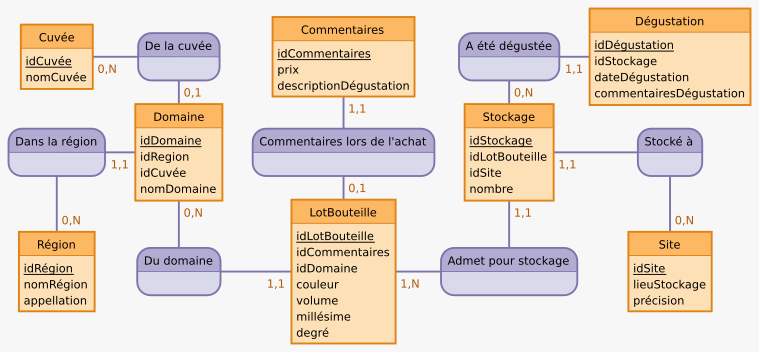
\includegraphics{Brigitte/Tp2_CaveVin/Tp2_CaveVin.png}
\caption{diagramme Brigitte}
\end{figure}

Description du schéma SQL :

\begin{Shaded}
\begin{Highlighting}[]
\NormalTok{PRAGMA foreign\_keys}\OperatorTok{=}\DecValTok{1}\NormalTok{;}

\KeywordTok{DROP} \KeywordTok{TABLE} \ControlFlowTok{if} \KeywordTok{EXISTS}\NormalTok{ Site;}
\KeywordTok{DROP} \KeywordTok{TABLE} \ControlFlowTok{if} \KeywordTok{EXISTS}\NormalTok{ Stockage;}
\KeywordTok{DROP} \KeywordTok{TABLE} \ControlFlowTok{if} \KeywordTok{EXISTS}\NormalTok{ Dégustation;}
\KeywordTok{DROP} \KeywordTok{TABLE} \ControlFlowTok{if} \KeywordTok{EXISTS}\NormalTok{ LotBouteille;}
\KeywordTok{DROP} \KeywordTok{TABLE} \ControlFlowTok{if} \KeywordTok{EXISTS}\NormalTok{ Région;}
\KeywordTok{DROP} \KeywordTok{TABLE} \ControlFlowTok{if} \KeywordTok{EXISTS}\NormalTok{ Domaine;}
\KeywordTok{DROP} \KeywordTok{TABLE} \ControlFlowTok{if} \KeywordTok{EXISTS}\NormalTok{ Cuvée; }
\KeywordTok{DROP} \KeywordTok{TABLE} \ControlFlowTok{if} \KeywordTok{EXISTS}\NormalTok{ Commentaires;}

\KeywordTok{CREATE} \KeywordTok{TABLE}\NormalTok{ Site(}
\NormalTok{    idSite }\DataTypeTok{INTEGER} \KeywordTok{NOT} \KeywordTok{NULL} \KeywordTok{PRIMARY} \KeywordTok{KEY}\NormalTok{,}
\NormalTok{    lieuStockage TXT,}
\NormalTok{    précision Stockage }\DataTypeTok{VARCHAR}\NormalTok{(}\DecValTok{1}\NormalTok{) }\KeywordTok{CHECK}\NormalTok{ (précision }\KeywordTok{IN}\NormalTok{ (}\StringTok{\textquotesingle{}H\textquotesingle{}}\NormalTok{,}\StringTok{\textquotesingle{}B\textquotesingle{}}\NormalTok{))}
\NormalTok{    );}

\KeywordTok{CREATE} \KeywordTok{TABLE}\NormalTok{ Stockage (}
\NormalTok{    idStockage }\DataTypeTok{INTEGER} \KeywordTok{NOT} \KeywordTok{NULL} \KeywordTok{PRIMARY} \KeywordTok{KEY}\NormalTok{,}
\NormalTok{    idLotBouteille }\DataTypeTok{INTEGER} \KeywordTok{NOT} \KeywordTok{NULL} \KeywordTok{REFERENCES}\NormalTok{ LotBouteille (idLotBouteille),}
\NormalTok{    idSite }\DataTypeTok{INTEGER} \KeywordTok{NOT} \KeywordTok{NULL} \KeywordTok{REFERENCES}\NormalTok{ SITE (idSite),}
\NormalTok{    nombre }\DataTypeTok{INTEGER} \KeywordTok{NOT} \KeywordTok{NULL}   \CommentTok{{-}{-} faire une somme sur différents sites contenant même bouteilles...}
\NormalTok{    );}

\KeywordTok{CREATE} \KeywordTok{TABLE}\NormalTok{ LotBouteille(}
\NormalTok{    idLotBouteille }\DataTypeTok{INTEGER} \KeywordTok{NOT} \KeywordTok{NULL} \KeywordTok{PRIMARY} \KeywordTok{KEY}\NormalTok{,}
\NormalTok{    idCommentaires }\DataTypeTok{INTEGER} \KeywordTok{NOT} \KeywordTok{NULL} \KeywordTok{REFERENCES}\NormalTok{ Commentaires(idCommentaires),}
\NormalTok{    idDomaine }\DataTypeTok{INTEGER} \KeywordTok{NOT} \KeywordTok{NULL} \KeywordTok{REFERENCES}\NormalTok{ Domaine(idDomaine),}
\NormalTok{    couleur }\DataTypeTok{VARCHAR}\NormalTok{(}\DecValTok{5}\NormalTok{) }\KeywordTok{CHECK}\NormalTok{(}\FunctionTok{LOWER}\NormalTok{(couleur) }\KeywordTok{IN}\NormalTok{ (}\StringTok{\textquotesingle{}rouge\textquotesingle{}}\NormalTok{,}\StringTok{\textquotesingle{}rose\textquotesingle{}}\NormalTok{,}\StringTok{\textquotesingle{}blanc\textquotesingle{}}\NormalTok{)),}
\NormalTok{    volume }\DataTypeTok{REAL} \KeywordTok{NOT} \KeywordTok{NULL} \KeywordTok{CHECK}\NormalTok{(volume }\OperatorTok{>=} \DecValTok{0}\NormalTok{),}
\NormalTok{    millésime }\DataTypeTok{INTEGER} \KeywordTok{CHECK}\NormalTok{(millésime }\OperatorTok{>=} \DecValTok{0}\NormalTok{),}
\NormalTok{    degré }\DataTypeTok{REAL} \KeywordTok{CHECK}\NormalTok{(degré }\OperatorTok{>=} \DecValTok{0}\NormalTok{)  }\CommentTok{{-}{-} Attention il faudra nettoyer \% °}
\NormalTok{    );}

\KeywordTok{CREATE} \KeywordTok{TABLE}\NormalTok{ Dégustation (}
\NormalTok{    idDégustation }\DataTypeTok{INTEGER} \KeywordTok{NOT} \KeywordTok{NULL} \KeywordTok{PRIMARY} \KeywordTok{KEY}\NormalTok{,}
\NormalTok{    idStockage }\DataTypeTok{INTEGER} \KeywordTok{NOT} \KeywordTok{NULL} \KeywordTok{REFERENCES}\NormalTok{ Stockage(idStockage),}
\NormalTok{    dateDégustation TXT,}
\NormalTok{    commentairesDégustation TXT }
\NormalTok{    );}

\KeywordTok{CREATE} \KeywordTok{TABLE}\NormalTok{ Région (}
\NormalTok{    idRégion }\DataTypeTok{INTEGER} \KeywordTok{NOT} \KeywordTok{NULL} \KeywordTok{PRIMARY} \KeywordTok{KEY}\NormalTok{,}
\NormalTok{    nomRégion TXT }\KeywordTok{NOT} \KeywordTok{NULL} \KeywordTok{UNIQUE}\NormalTok{,}
\NormalTok{    appellation TXT}
\NormalTok{    );}

\KeywordTok{CREATE} \KeywordTok{TABLE}\NormalTok{ Domaine (}
\NormalTok{    idDomaine }\DataTypeTok{INTEGER} \KeywordTok{NOT} \KeywordTok{NULL} \KeywordTok{PRIMARY} \KeywordTok{KEY}\NormalTok{,}
\NormalTok{    idRegion }\DataTypeTok{INTEGER} \KeywordTok{NOT} \KeywordTok{NULL} \KeywordTok{REFERENCES}\NormalTok{ Région(idRégion),}
\NormalTok{    idCuvée }\DataTypeTok{INTEGER} \KeywordTok{NOT} \KeywordTok{NULL} \KeywordTok{REFERENCES}\NormalTok{ Cuvée(idCuvée),}
\NormalTok{    nomDomaine TXT    }\CommentTok{{-}{-} un nom de domaine n\textquotesingle{}est pas forcément unique }
\NormalTok{    );}

\KeywordTok{CREATE} \KeywordTok{TABLE}\NormalTok{ Cuvée (}
\NormalTok{    idCuvée }\DataTypeTok{INTEGER} \KeywordTok{NOT} \KeywordTok{NULL} \KeywordTok{PRIMARY} \KeywordTok{KEY}\NormalTok{,}
\NormalTok{    nomCuvée TXT }\KeywordTok{UNIQUE}   \CommentTok{{-}{-}un nom de cuvée est unique mais peut être vide}
\NormalTok{    );}

\KeywordTok{CREATE} \KeywordTok{TABLE}\NormalTok{ Commentaires (}
\NormalTok{    idCommentaires }\DataTypeTok{INTEGER} \KeywordTok{NOT} \KeywordTok{NULL} \KeywordTok{PRIMARY} \KeywordTok{KEY}\NormalTok{,}
\NormalTok{    prix }\DataTypeTok{REAL} \KeywordTok{CHECK}\NormalTok{(prix }\OperatorTok{>=} \DecValTok{0}\NormalTok{),}
\NormalTok{    descriptionDégustation TXT}
\NormalTok{    );}
\end{Highlighting}
\end{Shaded}

    \hypertarget{correction}{%
\subsection{Correction}\label{correction}}

\textbf{ATTENTION : la proposition suivante est une base de discussion,
pas une correction absolue (s'il en existe une).}

\emph{Ce qui est peut-être le plus important sur cet exemple ou sur
votre proposition c'est d'être capable de comprendre et critiquer le
modèle, de déterminer les impacts de tel ou tel choix de modélisation.
Concrètement, cela signifie être capable de répondre à des questions
comme : un domaine peut-il produire plusieurs vins ? un vin peut t'il
être acheté plusieurs fois à des prix différents ? peut-on stocker un
même vin à différent endroits ? etc.}

\emph{Des choix faits dans cette proposition peuvent être discutés ad
nauseam et pour mettre fin aux discussions et avancer il faudra trancher
en accord avec le client. Une question d'apparence simple comme ``qu'est
ce qui permet d'identifier un vin'' n'est en fait pas évidente, donc que
le client nous le précise !}

Voir \href{cas_d_etude_modelisation.mcd}{le diagramme E/A JMerise} de la
proposition, \href{correction/cas_d_etude_modelisation.png}{sa
screenshot \texttt{png}}, et
\href{correction/cas_d_etude_modelisation.sql}{sa contrepartie SQL}. Le
SQL a été généré par JMerise et légèrement repris à la main.

\begin{figure}
\centering
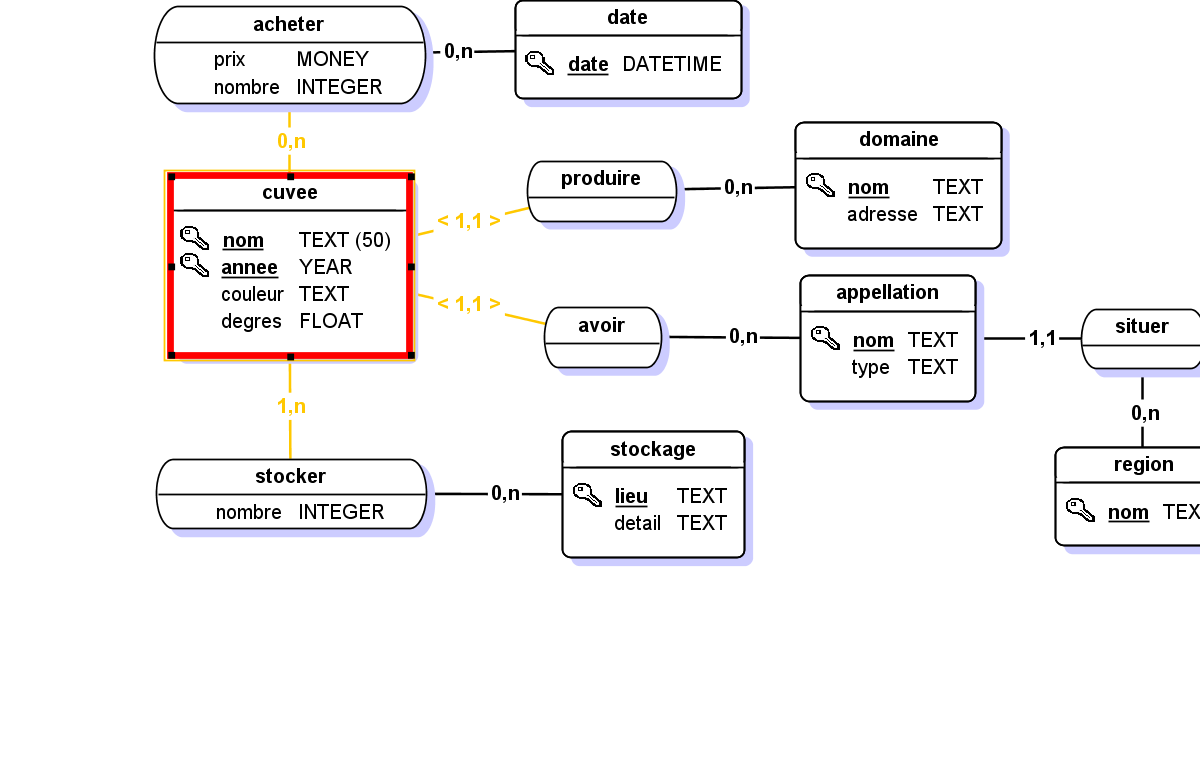
\includegraphics{correction/cas_d_etude_modelisation.png}
\caption{schéma}
\end{figure}

Quelques remarques :

\begin{itemize}
\tightlist
\item
  la région bénéficie de sa propre \emph{entité} mais \emph{couleur}
  n'est qu'un attribut (avec une contrainte \texttt{CHECK} dans le
  schéma SQL). En effet, on peut imaginer qu'on ait plus de choses à
  dire sur une région viticole (e.g., sa définition géographique) que
  sur la couleur du vin
\item
  le type de l'appellation (IGP, VdP, AOP) n'est souvent pas explicitée
  (e.g., ``Collinnes rhodaniennes'' est une IGP, ``Condrieu'' une AOP),
  il faudra compléter la base.
\end{itemize}

Le plus discutable est le choix \textbf{d'une cuvée millesimée} pour
représenter ``une bouteille'', ``un vin''. Ici, la \emph{cuvée} est une
\emph{entité faible} (dite aussi relative), c'est-à-dire que le
\emph{domaine} et \emph{l'appellation} \textbf{font partie de la clef}
de la \emph{cuvée} qui devient ainsi un quadruple :

\begin{itemize}
\tightlist
\item
  cela n'apparait pas dans l'exemple mais un producteur peut bien avoir
  plusieurs cuvées dont il a plusieurs millésimes pour une même
  appellation,
\item
  certaines bouteilles n'ont pas de cuvée spécifiée car le producteur ne
  produit qu'un seul vin par appellation, il faudra donc un nom par
  défaut (e.g., le nom de l'appellation, la chaine vide),
\item
  pour le champagne non millésimé, comme l'année fait partie de la clef,
  elle ne peut pas être nulle et il faudra faire un choix (e.g., l'année
  d'achat ou 1900), on aura le même problème si on souhaitait étendre
  aux alcools distillés
\end{itemize}

\textbf{Cette proposition de schéma a donc un \emph{impact} sur les
données car il faut, d'une façon ou d'une autre, remplir les colonnes où
il y a des trous dans la feuille de calcul avant d'importer dans la
base. Une autre proposition qui aurait comme postulat \emph{on ne doit
pas toucher aux données d'origine} aboutirait à un modèle
substentiellement différent, moins contraint.}

Une alternative à l'entité faible serait de tirer un identifiant qui
servirait de clef. C'est très prisé par les developpeurs, si ça
simplifie un peu la gestion de la clef (ici un quadruple), ça ne résoud
rien. Une autre prossibilité serait de distinguer \emph{cuvée} de
\emph{cuvée millésimée}, dans l'idée que la cuvée reste et que le
vigneron la produit, ou pas, d'une année sur l'autre.

\hypertarget{autres-questions}{%
\subsubsection{Autres questions}\label{autres-questions}}

Pour la qualité des données, on va s'attendre à des problèmes typiques
de données mal typées et saisies par des utilisateurs : unités variables
ou absentes dans les cases, cellules vides, erreur de saisies. Le plus
difficile étant le champs de \emph{l'appellation} où la variété des
saisies est importante (abbréviation, casse, orthographe etc.)

Pour l'historisation, il faut préciser ce que l'on veut, mais on
pourrait par exemple ajouter une nouvelle association \emph{degustation}
entre \emph{date} et \emph{cuvée} avec comme attribut un commentaire.
L'idée serait de remplir la table associée après destockage.


    % Add a bibliography block to the postdoc
    
    
    
    \end{document}
